\documentclass[openany]{article}
\usepackage[a4paper,margin=1in,bottom=1.5in]{geometry} % define margins. Bottom margin is used to lift a little bit the page number.
\usepackage[english]{babel} % document language is english
\usepackage{tikz} % for drawing (currently not used).
\usepackage{graphicx} % for including images
\usepackage[export]{adjustbox}
\usepackage{fancyhdr} % used for creating headers and footers. only used in title page in this document.
\usepackage{tabularx} % creation of more complex tables
\usepackage{longtable} % tables can span multiple pages
\usepackage{array} % allow elements of tabular environment to have vertical alignment, e.g., center alignment.
\usepackage{nameref} % make it possible to reference by name
\usepackage{hyperref} % allow hiperlinks (links to other document parts and extern links)
\usepackage{etoc} % used for generation of section local table of contents
\usepackage{placeins} % defines the \FloatBarrier command
\usepackage{xcolor} % for modifying box color
\usepackage{adjustbox} % for modifying box parameters
\usepackage{textcomp} % for having the degree symbol
\usepackage{listings} % for code snippets

% configure a listing environment for code snippets
\lstnewenvironment{code}
    {\lstset{linewidth=\linewidth,
             backgroundcolor=\color{white},
             frame=single,basicstyle=\normalsize\ttfamily\color{black},
             breaklines=true
             }}
    {}

% Define graphics path
\graphicspath{{figs/}}

% Configure the cross reference hyper links color
\hypersetup{
    colorlinks=true,
    linkcolor=blue,
}

\newcolumntype{C}{>{\centering\arraybackslash}X} % new column type for tabularx
                         % centered (\centering), adjust width in order to fill table width (X type)

% Configure header in 'titlepage'
\pagestyle{fancy}
\lhead{
\includegraphics[width=4.5cm]{logo_cnpem}}
\rhead{
\includegraphics[width=4cm]{logo_lnls}}
\renewcommand{\headrulewidth}{0pt}
\setlength{\headheight}{52pt}
% Clean footer
\fancyfoot{}

% increase table height factor a little bit (taller cells)
\renewcommand{\arraystretch}{1.5}

%==== Begin DOCUMENT ====
\begin{document}

%--- Begin title page ---
\begin{titlepage}

% Add header to this page
\thispagestyle{fancy}

% Center elements
\begin{center}

% title of title page
\topskip0pt % perfectly centered
\vspace*{\fill}
\textbf{\Huge Basler acA1300-75gm EPICS IOC User Guide}\\[20pt]
\textbf{\Huge Version 2.0}\\[20pt]
\textbf{\Huge April/2020}
\vspace*{\fill}

% footer of title page
\vfill
\textbf{Beam Diagnostics Group (DIGS)}\\[5pt]
\textbf{Brazilian Synchrotron Light Laboratory (LNLS)}\\[5pt]
\textbf{Brazilian Center for Research in Energy and Materials (CNPEM)}
\end{center}

\end{titlepage}
%--- End of title page ---

\newpage
\pagestyle{plain} % restore default page style

%--- About this manual ---
\paragraph{}{\Large\bfseries About this manual}

\paragraph{} This manual provides an overview of the Basler acA1300-75gm EPICS IOC support. It is assumed that the reader is familiar with the basics of EPICS.

%--- Table of contents ---
\tableofcontents

\newpage
%--- Section: Introduction ---
\section{Introduction}

\paragraph{} The Basler acA1300-75gm EPICS IOC is a software application for control and data acquisition of the acA1300-75gm camera through EPICS Process Variables (PVs). This IOC bundles, configures and simplifies the control of a range of \href{https://github.com/areaDetector/areaDetector}{areaDetector} modules and plugins, which were selected to provide features commonly required by the application, yet trying to keep the number of modules small. The IOC also makes use of an in-house areaDetector-based plugin module, \href{https://github.com/}{NDPluginDimFei}, which does gaussian fitting.

\paragraph{} The IOC repository is \url{https://github.com/lnls-dig/basler-acA1300-75gm-epics-ioc}.

%--- Section: Installation ---
\section{Installation}

    \paragraph{Requirements} This IOC has only been tested on x86-64 Linux distributions.

    \paragraph{Shortcut} It is possible to run a \emph{docker image} containing the IOC and all of its dependencies. This is advised if there is no problem in running your application from a container. Go to the \hyperref[sec:run-with-docker]{next section} to see how to do it.

    \subsection{Installing without docker}

        \paragraph{Before everything} Make sure you have EPICS Base 3.15 and synApps version 5.8 or later installed. If you want to install the required modules separately, instead of using synApps, here is a list:

        \begin{itemize}
          \item area detector R2-0 or later; recommended: R3-2
          \item asyn 4.26 (or later); recommended: R4-33
          \item autosave 5.6.1 (or later); recommended: R5-9
          \item busy 1.6.1 (or later); recommended: R1-7
          \item calc 3.4.2.1 (or later); recommended: R3-7
          \item sscan 2.10.1 (or later); recommended: R2-11-1
        \end{itemize} 

    \paragraph{} \textbf{The steps below assume a Linux x86-64 distribution. Please, use it as an example and make the necessary changes if you would like to use it for other architecture}.

        \subsubsection{Install basic libraries and tools needed by aravis}

            \vspace{1mm}
            \begin{code}
sudo apt-get update && \
apt-get install -y \
    intltool \
    libgirepository1.0-dev \
    gtk-doc-tools \
    libglib2.0-dev \
    libglibmm-2.4-dev
            \end{code}
            \vspace{1mm}

        \subsubsection{Install aravis}

            \vspace{1mm}
            \begin{code}
git clone https://github.com/lnls-dig/aravis.git /opt/aravis
cd /opt/aravis
git checkout ARAVIS_0_4_1-LNLS1
./autogen.sh
make distclean
            \end{code}
            \vspace{1mm}

        \subsubsection{Install aravisGigE}

            \vspace{1mm}
            \begin{code}
git clone https://github.com/lnls-dig/aravisGigE /opt/epics/aravisGigE
cd /opt/epics/aravisGigE
git checkout R2-1-LNLS2
echo 'EPICS_BASE=<EPICS Base path>' > configure/RELEASE.local
echo 'SUPPORT=<SynApps path>/support' >> configure/RELEASE.local
echo 'AREADETECTOR=<Area Detector path>' >> configure/RELEASE.local
echo 'ADCORE=$(AREADETECTOR)/ADCore' >> configure/RELEASE.local
echo 'ASYN=<Asyn Driver path>' >> configure/RELEASE.local
echo 'GLIBPREFIX=/usr' >> configure/RELEASE.local
echo 'GLIB_INC1=/usr/lib/x86-64-linux-gnu/glib-2.0/include' >> configure/RELEASE.local
echo 'GLIB_INC2=/usr/lib/x86-64-linux-gnu/glib-2.0/include' >> configure/RELEASE.local
sed -i '/USR_LIBS += glib-2.0/c\USR_SYS += glib-2.0' aravisGigEApp/src/Makefile
ln -s /opt/aravis vendor
make
            \end{code}
            \vspace{1mm}

        \subsubsection{Install ffmpegServer Plugin}

            \vspace{1mm}
            \begin{code}
sudo apt-get update && apt-get install -y unzip
git clone https://github.com/areaDetector/ffmpegServer.git /opt/epics/ffmpegServer
cd /opt/epics/ffmpegServer
git checkout 0f8341cb27ed97551b7cdbdd996a8b831251afaf
./install.sh
echo 'ARAVISGIGE=/opt/epics/aravisGigE' > configure/RELEASE.local
echo '-include $(ARAVISGIGE)/configure/RELEASE.local' >> configure/RELEASE.local
make
            \end{code}
            \vspace{1mm}

        \subsubsection{Install NDPluginDimFei \(Double Gaussian Fit\)}

            \vspace{1mm}
            \begin{code}
sudo apt-get update && \
apt-get install -y \
    liblapack3 \
    liblapack-dev \
    libopenblas-base \
    libopenblas-dev \
    liblapacke-dev
git clone https://github.com/lnls-dig/NDPluginDimFei.git /opt/epics/NDPluginDimFei
cd /opt/epics/NDPluginDimFei
git checkout v0.2.0
sed -i -e 's|^DIRS += install.*$|#DIRS += install|' Makefile
echo 'SUPPORT=<SynApps path>/support' > configure/RELEASE.local
echo '-include $(SUPPORT)/configure/RELEASE' >> configure/RELEASE.local
make
make install
            \end{code}
            \vspace{1mm}

        \subsubsection{Install basler-acA1300-75gm EPICS IOC}

            \vspace{1mm}
            \begin{code}
git clone https://github.com/lnls-dig/basler-acA1300-75gm-epics-ioc.git /opt/epics/basler-acA1300-75gm-epics-ioc
cd /opt/epics/basler-acA1300-75gm-epics-ioc
git checkout <COMMIT TAG>
echo 'ARAVISGIGE=/opt/epics/aravisGigE' > configure/RELEASE.local
echo '-include $(ARAVISGIGE)/configure/RELEASE.local' >> configure/RELEASE.local
echo 'FFMPEGSERVER=/opt/epics/ffmpegServer' >> configure/RELEASE.local
echo 'DIMFEI=/opt/epics/NDPluginDimFei' >> configure/RELEASE.local
echo 'CALC=$(SUPPORT)/calc-R3-7' >> configure/RELEASE.local
echo 'BUSY=$(SUPPORT)/busy-R1-7' >> configure/RELEASE.local
echo 'SSCAN=$(SUPPORT)/sscan-R2-11-1' >> configure/RELEASE.local
echo 'AUTOSAVE=$(SUPPORT)/autosave-R5-9' >> configure/RELEASE.local
echo 'HDF5_LIB = /usr/lib/x86_64-linux-gnu/hdf5/serial' >> configure/RELEASE.local
echo 'HDF5_INCLUDE = -I/usr/include/hdf5/serial' >> configure/RELEASE.local
echo 'SZIP_LIB = /usr/lib' >> configure/RELEASE.local
echo 'SZIP_INCLUDE =' >> configure/RELEASE.local
make
make install
            \end{code}
            \vspace{1mm}

%--- Section: Running the IOC from a docker container ---
\section{Running the IOC from a docker container}\label{sec:run-with-docker}

    \paragraph{} Make sure you have docker installed and that you understand the basics of creating, running and acessing a container, and downloading an image.

    \subsection{Downloading the image (IOC + dependencies)}

        \paragraph{} The image named \textbf{lnlsdig/basler-aca1300-75gm-epics-ioc} contains the compiled IOC and dependencies, and can be downloaded to your machine by running:

        \vspace{1mm}
        \begin{code}
docker pull lnlsdig/basler-aca-1300-75gm-epics-ioc:<IOC_TAG>
        \end{code}
        \vspace{1mm}

        where \emph{$<$IOC\_TAG$>$} should be replaced by the desired IOC version.

        \paragraph{} The IOC version list can be found at \url{https://hub.docker.com/r/lnlsdig/basler-aca1300-75gm-epics-ioc/tags}.

        After the IOC image is downloaded, you can instante it by running a container that uses it.

    \subsection{Running a docker container with that image}

        \paragraph{} One way to run the container is to do:

        \vspace{1mm}
        \begin{code}
docker run -it --network host --restart always --name <CONTAINER_NAME> lnlsdig/basler-aca-1300-75gm-epics-ioc:<IOC_TAG> -s <SERIAL_NUMBER> -P <PREFIX1> -R <PREFIX2>
        \end{code}
        \vspace{1mm}

        Which is going to run the container starting at its default entrypoint, that is, the IOC startup script. The parameter $<$IOC\_TAG$>$ should be replaced by the IOC version. All the arguments after it are passed to the IOC startup script when run in this way. The $<$SERIAL\_NUMBER$>$ argument is the serial number of camera that should be controlled, and $<$PREFIX1$>$ and $<$PREFIX2$>$ are the IOC EPICS PVs prefix, combined as follows: emph{PV\_PREFIX = PREFIX1 + PREFIX2}.

        \paragraph{} \textbf{If you run this command before downloading the image, the image is automatically downloaded, provided there is internet connection}.

        \paragraph{} Below you find an explanation for each flag we used in the above command.

        \begin{itemize}
          \item -it: interactive (STDIN open) and allocate pseudo-TTY. Since we did not change the container entrypoint, your terminal is going to connect to the IOC shell.
          \item --network host: configures the container to use the host's network stack inside the container. It is the simplest configuration to use, although it provides no isolation.
          \item --restart always: restarts the container automatically when it exits.
          \item --name $<$CONTAINER\_NAME$>$: configures the container name as $<$CONTAINER\_NAME$>$.
        \end{itemize}

        \paragraph{} In order to stop the docker container, i.e., the IOC, run:

        \vspace{1mm}
        \begin{code}
docker stop <CONTAINER_NAME>
        \end{code}
        \vspace{1mm}

        \paragraph{} If you want to delete the container, after stopping it, run:

        \vspace{1mm}
        \begin{code}
docker rm <CONTAINER_NAME>
        \end{code}
        \vspace{1mm}

        \paragraph{} You can also run the contaier with the \emph{--rm} flag to clean up the container and remove the file system when it exits.

    \subsection{Downloading the aravisGigE image only}

        \paragraph{} In case it is desirable to run an image with only aravis, aravisGigE and synApps modules installed, then the \textbf{lnlsdig/aravisgige-epics-module} image can be found at \url{https://hub.docker.com/r/lnlsdig/aravisgige-epics-module}, and downloaded by running:

        \vspace{1mm}
        \begin{code}
docker pull lnlsdig/aravisgige-epics-module:<TAG>
        \end{code}
        \vspace{1mm}

%--- Section: Running the IOC without docker ---
\section{Running the IOC without docker}

    After successfully building the IOC, from the IOC top directory, run:

        \vspace{1mm}
        \begin{code}
cd iocBoot/iocBasleracA130075gm &&
./runBasleracA130075gm.sh <options>
        \end{code}
        \vspace{1mm}

    The available options can be listed by passing any invalid option to the startup script, such as:

        \vspace{1mm}
        \begin{code}
./runBasleracA130075gm.sh -h
        \end{code}
        \vspace{1mm}

    or can be consulted in the README.md file at the IOC $<$TOP$>$ directory or project page \url{https://github.com/lnls-dig/basler-acA1300-75gm-epics-ioc}.

%--- Section: Control and Acquisition Overview ---
\section{Control and Acquisition Overview}

    \paragraph{} The following section describes the camera controls alongside images of the CS-Studio OPI user interface, which can be found in \emph{\textless TOP\textgreater\slash op\slash opi\slash basler.opi}. For a quick reference of the available PVs look at \hyperref[sec:process-variables]{Process Variables Description}.

    % OPI Overview and links
    \paragraph{} The image below shows an example of the IOC CS-Studio OPI. Each group in the OPI is associated to an index below, linking it to a description of its meaning and functionality.

    \begin{figure}[!h]
        \caption{OPI main view}
        \label{fig:opi-main}
        \centering
        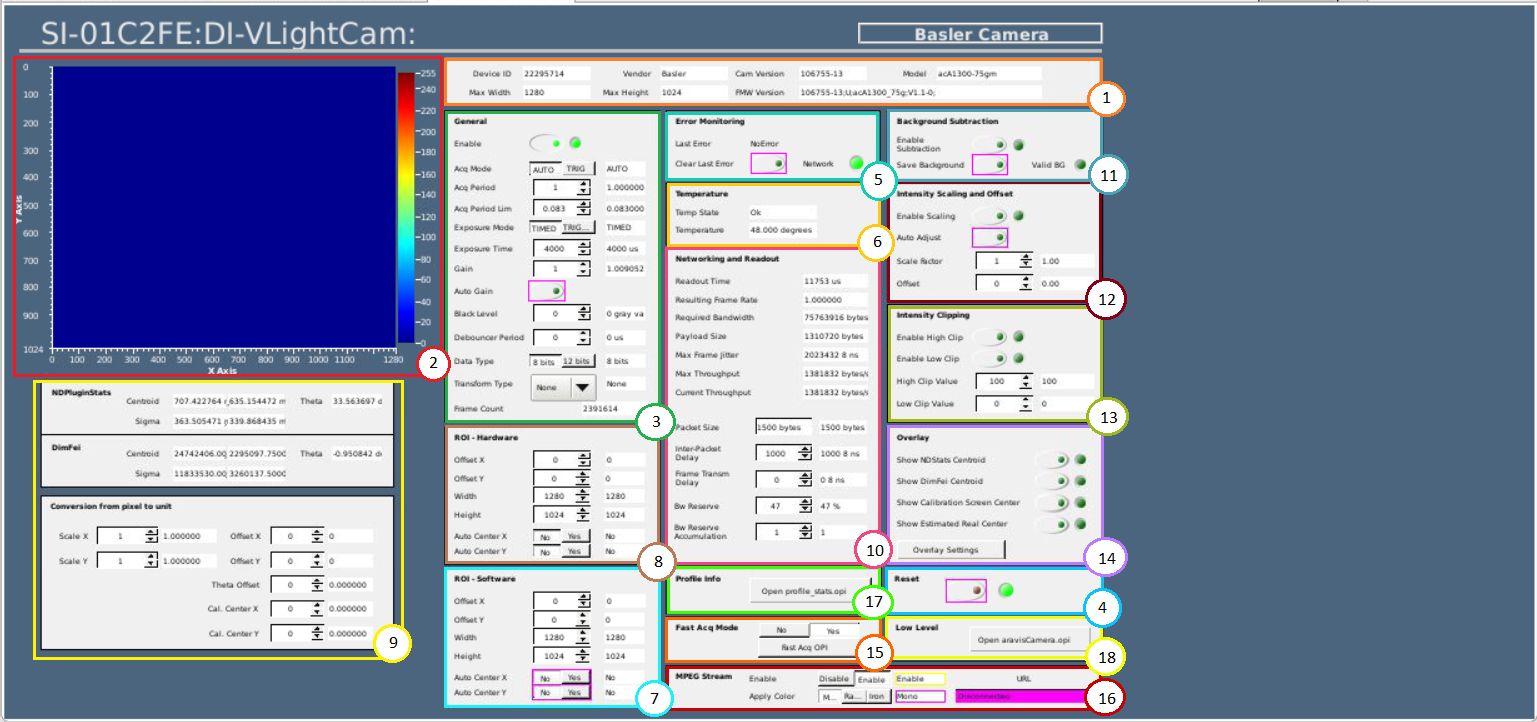
\includegraphics[width=1.0\textwidth]{example_opi_indexes}
    \end{figure}
    \FloatBarrier

    \begin{enumerate}
      \item \hyperref[sec:general-info]{Camera General Information}
      \item \hyperref[sec:image-data]{Image Data}
      \item \hyperref[sec:general-controls]{General Controls}
      \item \hyperref[sec:reset]{Reset}
      \item \hyperref[sec:err-mon]{Error Monitoring}
      \item \hyperref[sec:temp]{Temperature}
      \item \hyperref[sec:soft-roi]{Soft Region of Interest}
      \item \hyperref[sec:hard-roi]{Hard Region of Interest}
      \item \hyperref[sec:centroid-calc]{Centroid Calculation}
      \item \hyperref[sec:network-and-readout]{Network and Readout Settings}
      \item \hyperref[sec:background-sub]{Background Subtraction}
      \item \hyperref[sec:scaling]{Intensity Scaling and Offset}
      \item \hyperref[sec:clipping]{Intensity Clipping}
      \item \hyperref[sec:overlay]{Overlay}
      \item \hyperref[sec:fast-acq]{Fast Acquisition}
      \item \hyperref[sec:compressed-img]{Streaming Compressed Images}
      \item \hyperref[sec:profile-info]{Profile Information}
      \item \hyperref[sec:low-level-pvs]{Low Level OPI}
    \end{enumerate}

    %--- Section: Camera General Information ---
    \subsection{Camera General Information}\label{sec:general-info}

        \hyperref[fig:opi-main]{Return to Main OPI view}

        \begin{enumerate}
            \item \textbf{Device ID}: The device serial number.
                            Corresponding PV: \hyperlink{pv:device-id}{DeviceID-Cte}.
            \item \textbf{Sensor Width}: The width of the camera sensor in 
                            pixels. Corresponding PV: 
                            \hyperlink{pv:sensor-width}{SensorWidth-Cte}.
            \item \textbf{Sendor Height}: The height of the camera sensor in 
                            pixels. Corresponding PV: 
                            \hyperlink{pv:sensor-height}{SensorHeight-Cte}.
            \item \textbf{Vendor Name}: The camera vendor name. 
                            Corresponding PV: 
                            \hyperlink{pv:vendor-name}{DeviceVendorName-Cte}.
            \item \textbf{Device Version}: The version of the camera model.
                            Corresponding PV: 
                            \hyperlink{pv:device-version}{DeviceVersion-Cte}.
            \item \textbf{Device Model}: The camera model. 
                            Corresponding PV: 
                            \hyperlink{pv:device-model}{DeviceModelName-Cte}.
            \item \textbf{Firmware Version}: The camera firmware version.
                            Corresponding PV: 
                            \hyperlink{pv:firmware-version}{DeviceFirmwareVersion-Cte}.
        \end{enumerate}

    %--- Section: Image Data ---
    \subsection{Image Data}\label{sec:image-data}

        \hyperref[fig:opi-main]{Return to Main OPI view}

        \begin{enumerate}
            \item \textbf{Image Data}: The last frame acquired by the camera.
                            Corresponding PV: \hyperlink{pv:data-mon}{Data-Mon}.
        \end{enumerate}

    %--- Section: General Controls ---
    \subsection{General Controls}\label{sec:general-controls}

        \hyperref[fig:opi-main]{Return to Main OPI view}

        \paragraph{} The IOC main PVs can be found in the \emph{General} category in                             the OPI. The parameters available in this group are: 

        \begin{enumerate}
                    \item \textbf{Enable}: Enables camera acquisition. The camera must be 
                        disabled in order for changes to the hard ROI (AOI) size to be 
                        accepted. Changes to the high level ROI (SoftROI) size can be done 
                        while the camera is enabled. Corresponding PV: 
                        \hyperlink{pv:enbl}{Enbl-Sel/Sts}.
            \item \textbf{Acquisition Mode}: Configures the trigger type for 
                        acquisition start. In automatic mode, frames are continuously 
                        acquired, without the need of external triggers. In triggered mode,
                        a frame is acquired for each external trigger received by the 
                        camera. The triggers are only effective as long as the time interval
                        between them is greater than the value set for the acquisition 
                        period. Corresponding PV: \hyperlink{pv:acq-mode}{AcqMode-Sel/Sts}.
            \item \textbf{Acquisition Period}: This parameter defines the smaller 
                        time interval, in seconds, between frame acquisitions. In automatic
                        acquisition mode, the period between acquisitions is equal to the
                        acquisition period. Corresponding PV: 
                        \hyperlink{pv:acq-period}{AcqPeriod-SP/RB}.
            \item \textbf{Acquisition Period Limit}: This is a soft parameter used 
                        to set a warning associated to a given acquisition period. If the 
                        acquisition period is smaller than the acquisition period limit, 
                        than an alarm is raised for the acquisition period PV. Corresponding
                        PV: \hyperlink{pv:acq-period-lim}{AcqPeriodLowLim-SP/RB}.
            \item \textbf{Exposure Mode}: Configures whether the exposure period 
                        should be timed by the camera or be equal to the external trigger 
                        signal width. For example, if the camera is configured to timed 
                        exposure mode and the exposure period is configured to 5000 
                        microseconds, then, when the camera starts the acquisition of a 
                        frame, e.g., in response to an external trigger, the camera CCD 
                        sensor is going to be exposed to light for 5000 microseconds. If the
                        camera is configured to width exposure mode, the camera CCD is 
                        exposed while the external trigger signal is high, i.e., the 
                        exposure period has the length of the external trigger. The width 
                        mode can only be used when triggered acquisition mode is selected. 
                        Corresponding PV: \hyperlink{pv:exp-mode}{ExposureMode-Sel/Sts}.
            \item \textbf{Exposure Time}: Configures the exposure period, in 
                        microseconds. The configured period is only valid when the camera is
                        configured for timed exposure mode.
                        Corresponding PV: \hyperlink{pv:exp-time}{ExposureTime-SP/RB}.
            \item \textbf{Gain}: Configures the camera gain, in dB. Increasing gain 
                        increases camera sensitivity. Corresponding PV: 
                        \hyperlink{pv:gain}{Gain-SP/RB}.
            \item \textbf{Auto Gain}: Command to auto adjust camera gain using the 
                        last acquired frame. Corresponding PV: 
                        \hyperlink{pv:auto-gain}{AutoGain-Cmd}.
            \item \textbf{Black Level}: Configures a lower intensity threshold for 
                        the camera. Increasing the black level reduces the range of 
                        intensities that the camera detects. Corresponding PV: 
                        \hyperlink{pv:black-level}{BlackLevel-SP/RB}.
            \item \textbf{Debouncer Period}: Configures the external trigger 
                        debouncer period. An external trigger pulse must have at least the 
                        debouncer period duration in order to trigger the camera. Increasing
                        the debouncer period reduces the chance of noise triggering the 
                        camera. Corresponding PV: 
                        \hyperlink{pv:debouncer-period}{DebouncerPeriod-SP/RB}.
            \item \textbf{Data Type}: Configures the image color depth to 8 bits or
                        12 bits. The data type of the image waveform is, in both cases, 
                        USHORT. When 8-bits is selected, each image pixel can range from 0 
                        to 255. When 12-bits is selected, each pixel can range from 0 to 
                        65535. Although all 16 bits are used to represent the pixel 
                        intensity in the second configuration, they are in fact scaled to 
                        cover the entire range, providing still the same resolution as 12 
                        bits would. \hyperlink{pv:data-type}{DataType-Sel/Sts}.
             \item \textbf{Transform}: Configures rotation or mirror operations to 
                        the image. The rotation can only be applied in steps of 90 degrees.
                        The transformed image is the one used by centroid and profile 
                        statistics. For instance, the centroid position calculated can be 
                        changed if the image is rotated. Corresponding PV: 
                        \hyperlink{pv:transf-type}{TransformType-Sel/Sts}.
            \item \textbf{Frame Count}: Read-only monitor displaying the number of 
                        frames acquired since IOC start. Corresponding PV: 
                        \hyperlink{pv:frame-cnt}{FrameCnt-Mon}.
        \end{enumerate}

    %--- Section: Reset ---
    \subsection{Reset}\label{sec:reset}

        \hyperref[fig:opi-main]{Return to Main OPI view}

        \begin{enumerate}
            \item \textbf{Reset Command}: Resets the camera configuration and IOC 
                        driver. The connection is ended and automatically restablished. 
                        Correponding PV: \hyperlink{pv:reset}{Rst-Cmd}.
        \end{enumerate}

    %--- Section: Error Monitoring ---
    \subsection{Error Monitoring}\label{sec:err-mon}

        \hyperref[fig:opi-main]{Return to Main OPI view}

        \begin{enumerate}
            \item \textbf{Last Error}: Read-only monitor of the last error detected
                        by the camera. Corresponding PV: 
                        \hyperlink{pv:last-err}{LastErr-Mon}.
            \item \textbf{Clear Last Error}: Write-only command that erases the last
                        error detected by the camera. Corresponding PV: 
                        \hyperlink{pv:clear-last-err}{ClearLastErr-Cmd}.
            \item \textbf{Connection Status}: TCP connection status. Corresponding 
                        PV: \hyperlink{pv:connection}{Connection-Mon}.
        \end{enumerate}

    %--- Section: Temperature ---
    \subsection{Temperature}\label{sec:temp}

        \hyperref[fig:opi-main]{Return to Main OPI view}

        \begin{enumerate}
            \item \textbf{Temperature State}: Indicates whether the device temperature is acceptable. Corresponding PV: \hyperlink{pv:temp-state}{TempState-Mon}.
            \item \textbf{Temperature}: Indicates the device current temperature. Corresponding PV: \hyperlink{pv:temp}{Temp-Mon}.
        \end{enumerate}

    %--- Section: Soft Region of Interest ---
    \subsection{Soft Region of Interest}\label{sec:soft-roi}

        \hyperref[fig:opi-main]{Return to Main OPI view}

        \paragraph{} The Soft ROI controls the output image size by discarding unnecessary data. It also decouples the image ROI from the rotation and mirror configurations, making it simpler for other plugins to account for ROI changes (see also \hyperref[sec:hard-roi]{Hard ROI}). It is NOT necessary to stop acquisition to make changes to Soft ROI configurations. Changes to the Soft ROI are also automatically accounted by \hyperref[sec:centroid-calc]{Centroid Calculation}.

        \paragraph{} Soft ROI parameters:

        \begin{enumerate}
            \item \textbf{Soft ROI Offset X}: Defines the ROI offset, in pixels, in the X axis, from left to right. Corresponding PV: \hyperlink{pv:soft-roi-off-x}{SoftROIOffsetX-SP/RB}.
            \item \textbf{Soft ROI Offset Y}: Defines the ROI offset, in pixels, in the Y axis, from top to bottow. Corresponding PV: \hyperlink{pv:soft-roi-off-y}{SoftROIOffsetY-SP/RB}.
            \item \textbf{Soft ROI Width}: Defines the ROI width, in pixels. Corresponding PV: \hyperlink{pv:soft-roi-width}{SoftROIWidth-SP/RB}.
            \item \textbf{Soft ROI Height}: Defines the ROI height, in pixels. Corresponding PV: \hyperlink{pv:soft-roi-height}{SoftROIHeight-SP/RB}.
            \item \textbf{Soft ROI Auto Center X}: When enabled, the X offset is automatically adjusted to centralize the ROI with respect to the camera whenever the ROI size is changed. Corresponding PV: \hyperlink{pv:soft-roi-auto-center-x}{SoftROIAutoCenterX-Sel/Sts}.
            \item \textbf{Soft ROI Auto Center Y}: When enabled, the Y offset is automatically adjusted to centralize the ROI with respect to the camera whenever the ROI size is changed. Corresponding PV: \hyperlink{pv:soft-roi-auto-center-y}{SoftROIAutoCenterY-Sel/Sts}.
        \end{enumerate}

    %--- Section: Hard Region of Interest ---
    \subsection{Hard Region of Interest}\label{sec:hard-roi}

        \hyperref[fig:opi-main]{Return to Main OPI view}

        \paragraph{} The Hard ROI (AOI) controls the size of the image which is sent by the camera to the IOC. This parameter is useful when trying to reduce the network bandwidth consumption, by sending a smaller region of interest. Changes to the Hard ROI require the \hyperref[sec:centroid-calc]{Centroid Calculation} to be recalibrated, in order to agree with the new ROI settings.

        \paragraph{}Hard ROI parameters:

        \begin{enumerate}
            \item \textbf{Hard ROI Offset X}: Defines the Hard ROI offset in the X axis, in pixels, from left to right. This configuration is not aware of rotation and mirror settings, which are applied by the IOC and not by the camera. Changing the X offset with the image rotated may change the output image Y axis instead, therefore the transformation setting (\emph{TransformType-Sts}) should be checked before making changes to the Hard ROI position. Corresponding PV: \hyperlink{pv:hard-roi-off-x}{AOIOffsetX-SP/RB}.
            \item \textbf{Hard ROI Offset Y}: Defines the Hard ROI offset in the Y axis, in pixels, from top to bottow. This configuration is not aware of rotation and mirror settings, which are applied by the IOC and not by the camera. Changing the Y offset with the image rotated may change the output image X axis instead, therefore the transformation setting (\emph{TransformType-Sts}) should be checked before making changes to the Hard ROI position. Corresponding PV: \hyperlink{pv:hard-roi-off-y}{AOIOffsetY-SP/RB}.
            \item \textbf{Hard ROI Width}: Defines the Hard ROI width. This configuration is not aware of the rotation setting, which is applied by the IOC and not by the camera. Changing the ROI width with the image rotated may change the output image height instead, therefore the transformation setting (\emph{TransformType-Sts}) should be checked before making changes to the Hard ROI size. Corresponding PV: \hyperlink{pv:hard-roi-width}{AOIWidth-SP/RB}.
            \item \textbf{Hard ROI Height}: Defines the Hard ROI height. This configuration is not aware of the rotation setting, which is applied by the IOC and not by the camera. Changing the ROI height with the image rotated may change the output image width instead, therefore the transformation setting (\emph{TransformType-Sts}) should be checked before making changes to the Hard ROI size. Corresponding PV: \hyperlink{pv:hard-roi-height}{AOIHeight-SP/RB}.
            \item \textbf{Hard ROI Auto Center X}: When auto center X is enabled, the Hard ROI X offset is automatically adjusted to centralize the ROI with respect to the camera whenever the ROI size is changed. This configuration is not aware of the rotation setting, which is applied by the IOC and not by the camera. Make sure to check the transformation setting (\emph{TransformType-Sts}). Corresponding PV: \hyperlink{pv:hard-roi-auto-center-x}{AOIAutoCenterX-Sel/Sts}.
            \item \textbf{Hard ROI Auto Center Y}: When auto center Y is enabled, the Hard ROI Y offset is automatically adjusted to centralize the ROI with respect to the camera whenever the ROI size is changed. This configuration is not aware of the rotation setting, which is applied by the IOC and not by the camera. Make sure to check the transformation setting (\emph{TransformType-Sts}). Corresponding PV: \hyperlink{pv:hard-roi-auto-center-y}{AOIAutoCenterY-Sel/Sts}.
        \end{enumerate}

    %--- Section: Centroid Calculation ---
    \subsection{Centroid Calculation}\label{sec:centroid-calc}

        \hyperref[fig:opi-main]{Return to Main OPI view}

        \begin{enumerate}
            \item \textbf{NDStats Centroid Threshold}: Set the threshold value used when computing the centroid position and size with NDPluginStats. Pixel values smaller than the threshold are set to zero before the calculation. Enabling \hyperref[seq:fast-acq]{Fast Acquisition} disables centroid calculation. Corresponding PV: \hyperlink{pv:centroid-threshold-ndstats}{CentroidThresholdNDStats-SP}.
            \item \textbf{NDStats Centroid Center X}: Image centroid X as calculated by the NDStats plugin. NDStats calculates the centroid using image moments, and does so automatically anytime a new image is received from the camera. Enabling \hyperref[seq:fast-acq]{Fast Acquisition} disables centroid calculation. Corresponding PV: \hyperlink{pv:center-x-ndstats}{CenterXNDStats-Mon}.
            \item \textbf{NDStats Centroid Center Y}: Image centroid Y as calculated by the NDStats plugin. NDStats calculates the centroid using image moments, and does so automatically anytime a new image is received from the camera. Enabling \hyperref[seq:fast-acq]{Fast Acquisition} disables centroid calculation. Corresponding PV: \hyperlink{pv:center-y-ndstats}{CenterYNDStats-Mon}.
            \item \textbf{NDStats Centroid Sigma X}: Image centroid sigma X as calculated by the NDStats plugin. NDStats calculates the centroid using image moments, and does so automatically anytime a new image is received from the camera. Enabling \hyperref[seq:fast-acq]{Fast Acquisition} disables centroid calculation. Corresponding PV: \hyperlink{pv:sigma-x-ndstats}{SigmaXNDStats-Mon}.
            \item \textbf{NDStats Centroid Sigma Y}: Image centroid sigma Y as calculated by the NDStats plugin. NDStats calculates the centroid using image moments, and does so automatically anytime a new image is received from the camera. Enabling \hyperref[seq:fast-acq]{Fast Acquisition} disables centroid calculation. Corresponding PV: \hyperlink{pv:sigma-y-ndstats}{SigmaYNDStats-Mon}.
            \item \textbf{NDStats Centroid Sigma XY}: Image centroid normalized sigma XY, or correlation coefficient, as calculated by the NDStats plugin. NDStats calculates the centroid using image moments, and does so automatically anytime a new image is received from the camera. Enabling \hyperref[seq:fast-acq]{Fast Acquisition} disables centroid calculation. Corresponding PV: \hyperlink{pv:sigma-x-ndstats}{SigmaXYNDStats-Mon}.
            \item \textbf{NDStats Centroid Theta}: Image centroid angle as calculated by the NDStats plugin. NDStats calculates the centroid using image moments, and does so automatically anytime a new image is received from the camera. Enabling \hyperref[seq:fast-acq]{Fast Acquisition} disables centroid calculation. Corresponding PV: \hyperlink{pv:theta-ndstats}{ThetaNDStats-Mon}.
            \item \textbf{DimFei Centroid Center X}: Image centroid X as calculated by the DimFei plugin. DimFei calculates the centroid using double gaussian fit, and does so automatically anytime a new image is received from the camera. Enabling \hyperref[seq:fast-acq]{Fast Acquisition} disables centroid calculation. Corresponding PV: \hyperlink{pv:center-x-dimfei}{CenterXDimFei-Mon}.
            \item \textbf{DimFei Centroid Center Y}: Image centroid Y as calculated by the DimFei plugin. DimFei calculates the centroid using double gaussian fit, and does so automatically anytime a new image is received from the camera. Enabling \hyperref[seq:fast-acq]{Fast Acquisition} disables centroid calculation. Corresponding PV: \hyperlink{pv:center-y-dimfei}{CenterYDimFei-Mon}.
            \item \textbf{DimFei Centroid Sigma X}: Image centroid sigma X as calculated by the DimFei plugin. DimFei calculates the centroid using double gaussian fit, and does so automatically anytime a new image is received from the camera. Enabling \hyperref[seq:fast-acq]{Fast Acquisition} disables centroid calculation. Corresponding PV: \hyperlink{pv:sigma-x-dimfei}{SigmaXDimFei-Mon}.
            \item \textbf{DimFei Centroid Sigma Y}: Image centroid sigma Y as calculated by the DimFei plugin. DimFei calculates the centroid using double gaussian fit, and does so automatically anytime a new image is received from the camera. Enabling \hyperref[seq:fast-acq]{Fast Acquisition} disables centroid calculation. Corresponding PV: \hyperlink{pv:sigma-y-dimfei}{SigmaYDimFei-Mon}.
            \item \textbf{DimFei Centroid Theta}: Image centroid angle as calculated by the DimFei plugin. DimFei calculates the centroid using double gaussian fit, and does so automatically anytime a new image is received from the camera. Enabling \hyperref[seq:fast-acq]{Fast Acquisition} disables centroid calculation. Corresponding PV: \hyperlink{pv:theta-dimfei}{ThetaDimFei-Mon}.
            \item \textbf{Centroid Scale X}: Scaling factor at the X axis for centroid statistics. Centroid statistics default unit is pixel. In order to convert the results to another unit a conversion factor is required. Corresponding PV: \hyperlink{pv:scale-factor-x}{ScaleFactorX-SP/RB}.
            \item \textbf{Centroid Scale Y}: Scaling factor at the Y axis for centroid statistics. Centroid statistics default unit is pixel. In order to convert the results to another unit a conversion factor is required. Corresponding PV: \hyperlink{pv:scale-factor-y}{ScaleFactorY-SP/RB}.
            \item \textbf{Image Desired Reference Offset X}: Offset in the X axis, in pixels, of the desired reference position with respect to the raw image origin, i.e., the topmost, leftmost image corner. The offset cannot be negative. This value is used to calculate the centroid position with respect to the desired reference, instead of the raw image origin (default). The desired reference position will often be indicated by a \emph{Calibration Screen} positioned at the right position in front of the camera. Corresponding PV: \hyperlink{pv:center-offset-x}{CenterOffsetX-SP/RB}.
            \item \textbf{Image Desired Reference Offset Y}: Offset in the Y axis, in pixels, of the desired reference position with respect to the raw image origin, i.e., the topmost, leftmost image corner. The offset cannot be negative. This value is used to calculate the centroid position with respect to the desired reference, instead of the raw image origin (default). The desired reference position will often be indicated by a \emph{Calibration Screen} positioned at the right position in front of the camera. Corresponding PV: \hyperlink{pv:center-offset-y}{CenterOffsetY-SP/RB}.
            \item \textbf{Image Desired Reference Theta Offset}: Angular offset of the desired image reference axes with respect to the raw image axes. This value is used to calculate the centroid rotation with respect to the desired reference, instead of the raw image axes (default). This is useful for compensating unwanted camera rotation. The desired reference angle will often be indicated by a \emph{Calibration Screen} positioned at the right point in front of the camera. Clockwise rotation is expressed with a positive sign (+), while counterclockwise rotation with a negative one (-). Corresponding PV: \hyperlink{pv:theta-offset}{ThetaOffset-SP/RB}.
            \item \textbf{Image Desired Reference Coordinate X}: Desired reference real-world X coordinate. By default, the desired reference position indicates the origin (0,0) of the coordinate system in which the centroid coordinates are expressed. But the reference position can actually express any position in the desired reference frame. This allows, for instance, for compensation of alignment problems in a \emph{Calibration Screen}. When the misalignment is measurable, the true Screen position can be entered in the coordinates X and Y of the desired reference. Corresponding PV: \hyperlink{pv:cal-pos-center-x}{CalPosCenterX-SP/RB}.
            \item \textbf{Image Desired Reference Coordinate Y}: Desired reference real-world Y coordinate. By default, the desired reference position indicates the origin (0,0) of the coordinate system in which the centroid coordinates are expressed. But the reference position can actually express any position in the desired reference frame. This allows, for instance, for compensation of alignment problems in a \emph{Calibration Screen}. When the misalignment is measurable, the true Screen position can be entered in the coordinates X and Y of the desired reference. Corresponding PV: \hyperlink{pv:cal-pos-center-y}{CalPosCenterY-SP/RB}.
        \end{enumerate}

    %--- Section: Network and Readout ---
    \subsection{Network and Readout Settings}\label{sec:network-and-readout}

        \hyperref[fig:opi-main]{Return to Main OPI view}

        \begin{enumerate}
            \item \textbf{Readout Time} The readout time is the period the camera takes to read the pixel values after the exposure period is finished. The sensor readout time is the sum of each sensor line readout time and therefore depends on the AOI height. Corresponding PV: \hyperlink{pv:readout-time}{ReadoutTime-Mon}.
            \item \textbf{Resulting Frame Rate} This parameter indicates the maximum allowed frame rate given the camera current settings. Corresponding PV: \hyperlink{pv:result-frame-rate}{ResultFrameRate-Mon}.
            \item \textbf{Bandwidth Assigned} This parameter indicates the total bandwidth, in bytes per second, that will be used to transmit image data and handle resends and transmission control. This parameter is a result of the packet size and the inter-packet delay settings. Corresponding PV: \hyperlink{pv:bw-assigned}{BwAssigned-Mon}.
            \item \textbf{Payload Size} Indicates the size, in bytes, of the image data, not including packet headers. Corresponding PV: \hyperlink{pv:payload-size}{PayloadSize-Mon}.
            \item \textbf{Max Frame Jitter} Indicates the maximum time, in ticks of 8 ns intervals, that a transmission could be delayed due to a burst of resends (maximum number of resends is limited by \emph{Bandwidth Reserve Accumulation}). Corresponding PV: \hyperlink{pv:frame-max-jitter}{FrameMaxJitter-Mon}.
            \item \textbf{Data Max Throughput} Indicates the maximum amount of data that the camera could generate given no network restrictions or packet resends. If automatic periodic acquisition is been used, the camera will use the frame rate setting to calculate the max throughput. If software or hardware triggering is being used, the max frame rate allowed with the current camera settings will be used to calculate the max throughput. Corresponding PV: \hyperlink{pv:max-throughput}{MaxThroughput-Mon}.
            \item \textbf{Data Current Throughput} Indicates the bandwidth that the camera will need to transmit the image data given the current area of interest and pixel format, without considering bandwidth reserved for retries and needed for overhead, such as leaders and trailers. Corresponding PV: \hyperlink{pv:current-throughput}{CurrentThroughput-Mon}.
            \item \textbf{Packet Size} This parameter sets the size of packets used to transmit the data payload. The packet payload is equal to packet size minus 36 bytes from leader and trailer. The packet size should be set to the maximum size that the network adapter and switches can handle. Corresponding PV: \hyperlink{pv:packet-size}{PacketSize-SP/RB}.
            \item \textbf{Inter-packet Delay} This parameter sets the delay, in ticks of 8 ns, between packets. Corresponding PV: \hyperlink{pv:inter-packet-delay}{InterPacketDelay-SP/RB}.
            \item \textbf{Transmission Delay} This parameter sets the delay, in ticks of 8 ns, between the time when the camera becomes ready to transmit a frame and when it actually begins to transmit it. Corresponding PV: \hyperlink{pv:transm-delay}{TransmDelay-SP/RB}.
            \item \textbf{Bandwidth Reserve} This parameter defines the percentage of the assigned bandwidth to be used for packet resends and transmission of control data between camera and host computer. Corresponding PV: \hyperlink{pv:bw-reserve}{BwReserve-SP/RB}.
            \item \textbf{Bandwidth Reserve Accumulation} After an unusual problem that interrupts image transmission, such as an EMI burst, the camera can use a larger than normal number of resends to transmit the complete image. This parameter is a multiplier to the \emph{Bandwidth Reserve} that limits the maximum number of resends that can be held in the accumulator pool. Corresponding PV: \hyperlink{pv:bw-reserve-accum}{BwReserveAccum-SP/RB}.
        \end{enumerate}

    %--- Section: Background Subtraction ---
    \subsection{Background Subtraction}\label{sec:background-sub}

        \hyperref[fig:opi-main]{Return to Main OPI view}

        \begin{enumerate}
            \item \textbf{Enable Background Subtraction} This PV enables/disables background subtraction, i.e., if there is a valid background saved, it is subtracted from acquired frames. Corresponding PV: \hyperlink{pv:enbl-bg-subtraction}{EnblBGSubtraction-Sel/Sts}.
            \item \textbf{Save Background} Save background command. After the command is issued, the next acquired frame is saved as background. Corresponding PV: \hyperlink{pv:save-bg}{SaveBG-Cmd}.
            \item \textbf{Valid Background} Indicates whether there is a valid background saved. Corresponding PV: \hyperlink{pv:valid-bg}{ValidBG-Mon}.
        \end{enumerate}

    %--- Section: Intensity Scaling and Offset ---
    \subsection{Intensity Scaling and Offset}\label{sec:scaling}

        \hyperref[fig:opi-main]{Return to Main OPI view}

        \begin{enumerate}
            \item \textbf{Enable Intensity Offset and Scale} Enables offset and scale for the pixel intensity values. These operations cannot improve the image SNR, but can make it easier to see images with too low intensity. Corresponding PV: \hyperlink{pv:enbl-offset-scale}{EnblOffsetScale-Sel/Sts}.
            \item \textbf{Auto Adjust Intensity Offset and Scale} When pixel intensity offset and scale is enabled, this command auto adjusts offset and scale so that the image intensity range fills the entire available range. Corresponding PV: \hyperlink{pv:auto-offset-scale}{AutoOffsetScale-Cmd}.
            \item \textbf{Pixel Intensity Scale} This parameter value is multiplier to each image pixel value. Corresponding PV: \hyperlink{pv:pixel-scale}{PixelScale-SP/RB}.
            \item \textbf{Pixel Intensity Offset} This parameter value is an offset added to each image pixel value. Corresponding PV: \hyperlink{pv:pixel-offset}{PixelOffset-SP/RB}.
        \end{enumerate}

    %--- Section: Intensity Clipping ---
    \subsection{Intensity Clipping}\label{sec:clipping}

        \hyperref[fig:opi-main]{Return to Main OPI view}

        \begin{enumerate}
            \item \textbf{Enable High Clip} When High Clip is enabled, pixel values greater than the \emph{High Clip value} are made equal to it. Corresponding PV: \hyperlink{pv:enbl-high-clip}{EnblHighClip-Sel/Sts}.
            \item \textbf{High Clip Value} This parameter is the High Clip limit value. When High Clip is enabled, values greater than the limit are made equal to it. Corresponding PV: \hyperlink{pv:high-clip}{HighClip-SP/RB}.
            \item \textbf{Enable Low Clip}  When Low Clip is enabled, pixel values smaller than the \emph{Low Clip Value} are made equal to it. Corresponding PV: \hyperlink{pv:enbl-low-clip}{EnblLowClip-Sel/Sts}.
            \item \textbf{Low Clip Value} This parameter is the Low Clip limit value. When Low Clip is enabled, values smaller than the limit are made equal to it. Corresponding PV: \hyperlink{pv:low-clip}{LowClip-SP/RB}.
        \end{enumerate}

    %--- Section: Overlay ---
    \subsection{Overlay}\label{sec:overlay}

        \hyperref[fig:opi-main]{Return to Main OPI view}

        \begin{enumerate}
            \item \textbf{Enable Marker Overlay for NDStats Centroid} Enables the overlay marker for NDStats centroid. After the marker is enabled, newly acquired frames receive the marker overlay. COrresponding PV: \hyperlink{pv:ndstats-mark-enbl}{NDStatsMarkEnbl-Sel/Sts}.
            \item \textbf{Size of NDStats Centroid Marker} Sets the size, in pixels, of the NDStats centroid marker. Corresponding PV: \hyperlink{pv:ndstats-mark-size}{NDStatsMarkSize-SP/RB}.
            \item \textbf{Color of NDStats Centroid Marker} Sets the gray value of the NDStats centroid marker. Corresponding PV: \hyperlink{pv:ndstats-mark-color}{NDStatsMarkColor-SP/RB}.
            \item \textbf{Enable Marker Overlay for DimFei Centroid} Enables the overlay marker for DimFei centroid. After the marker is enabled, newly acquired frames receive the marker overlay. Corresponding PV: \hyperlink{pv:dimfei-mark-enbl}{DimFeiMarkEnbl-Sel/Sts}.
            \item \textbf{Size of DimFei Centroid Marker} Sets the size, in pixels, of the DimFei centroid marker. Corresponding PV: \hyperlink{pv:dimfei-mark-size}{DimFeiMarkSize-SP/RB}.
            \item \textbf{Color of DimFei Centroid Marker} Sets the gray value of the DimFei centroid marker. Corresponding PV: \hyperlink{pv:dimfei-mark-color}{DimFeiMarkColor-SP/RB}.
            \item \textbf{Enable Marker Overlay for Reference Position} Enables the overlay marker for Reference Position. After the marker is enabled, newly acquired frames receive the marker overlay. Corresponding PV: \hyperlink{pv:cal-center-mark-enbl}{CalCenterMarkEnbl-Sel/Sts}.
            \item \textbf{Size of Reference Position Marker} Sets the size, in pixels, of the Reference Position marker. Corresponding PV: \hyperlink{pv:cal-center-mark-size}{CalCenterMarkSize-SP/RB}.
            \item \textbf{Color of Reference Position Marker} Sets the gray value of the Reference Position marker. Corresponding PV: \hyperlink{pv:cal-center-mark-color}{CalCenterMarkColor-SP/RB}.
            \item \textbf{Enable Marker Overlay for Real Center Position} Enables the overlay marker for Real Center Position. After the marker is enabled, newly acquired frames receive the marker overlay. Corresponding PV: \hyperlink{pv:real-center-mark-enbl}{RealCenterMarkEnbl-Sel/Sts}.
            \item \textbf{Size of Real Center Position Marker} Sets the size, in pixels, of the Real Center Position marker. Corresponding PV: \hyperlink{pv:real-center-mark-size}{RealCenterMarkSize-SP/RB}.
            \item \textbf{Color of Real Center Position Marker} Sets the gray value of the Real Center Position marker. Corresponding PV: \hyperlink{pv:real-center-mark-color}{RealCenterMarkColor-SP/RB}.
        \end{enumerate}

    %--- Section: Fast Acquisition ---
    \subsection{Fast Acquisition}\label{sec:fast-acq}

        \hyperref[fig:opi-main]{Return to Main OPI view}

        \begin{enumerate}
            \item \textbf{Enable Fast Acquisition Mode} The purpose of the \emph{fast acquisition mode} is to allow larger frame rates compared to normal acquisition, while keeping CPU usage and dropped frame count as small as possible. When fast acquisition is enabled, all of the plugins in the main image processing chain are disabled and the raw image is directly forwarded to the \emph{NDPluginStdArrays} plugin, which converts it to an epics waveform. Note that when fast acquisition is enabled, many IOC features will NOT work, such as Centroid Calculation, Image rotation and mirroring, Soft ROI, Background Subtraction, Intensity Scaling and Offset, Intensity Clipping, and Overlays. The ffmpeg image compression server and color conversion for the MJPG stream continue to work, however it is recommeded to disable color conversion, since it can cause dropped frames. Corresponding PV: \hyperlink{pv:fast-acq}{FastAcq-Sel/Sts}.
        \end{enumerate}

    %--- Section: Streaming Compressed Images ---
    \subsection{Streaming Compressed Images}\label{sec:compressed-img}

        \hyperref[fig:opi-main]{Return to Main OPI view}

        \begin{enumerate}
            \item \textbf{Enable MJPG Server} Enables image compression. When image compression is enabled, a copy of the camera raw image is compressed to MJPEG and made available by an HTTP server at the URL informed by the \emph{MJPGURL-Cte} PV. Corresponding PV: \hyperlink{pv:enbl-mjpeg}{EnblMJPEG-Sel/Sts}.
            \item \textbf{Enable Color Convertion} Enables color conversion for the MJPG stream, from monochrome to some of the predefined palettes. Corresponding PV: \hyperlink{pv:color-conv}{ColorConv-Sel/Sts}.
            \item \textbf{MJPG Server URL} URL of the MJPG stream. Corresponding PV: \hyperlink{pv:mjpg-url}{MJPGURL-Cte}.
        \end{enumerate}

    %--- Section: Profile Information ---
    \subsection{Profile Information}\label{sec:profile-info}

        \hyperref[fig:opi-main]{Return to Main OPI view}

        \begin{enumerate}
            \item \textbf{Enable Profile Calculation} Corresponding PV: \hyperlink{pv:profile-enbl}{ProfileEnbl-Sel/Sts}.
            \item \textbf{Profile ROI X Axis Offset} Corresponding PV: \hyperlink{pv:profile-roi-offset-x}{ProfileROIOffsetX-SP/RB}.
            \item \textbf{Profile ROI Y Axis Offset} Corresponding PV: \hyperlink{pv:profile-roi-offset-y}{ProfileROIOffsetY-SP/RB}.
            \item \textbf{Profile ROI Width} Corresponding PV: \hyperlink{pv:profile-roi-width}{ProfileROIWidth-SP/RB}.
            \item \textbf{Profile ROI Height} Corresponding PV: \hyperlink{pv:profile-roi-height}{ProfileROIHeight-SP/RB}.
            \item \textbf{Profile Cursor X Position} Position of X cursor for vertical profile computation. Corresponding PV: \hyperlink{pv:profile-cursor-x}{ProfileCursorX-SP/RB}.
            \item \textbf{Profile Cursor Y Position} Position of Y cursor for horizontal profile computation. Corresponding PV: \hyperlink{pv:profile-cursor-y}{ProfileCursorY-SP/RB}.
            \item \textbf{Horizontal Profile} Horizontal profile at cursor Y. Corresponding PV: \hyperlink{pv:profile-h}{ProfileH-Mon}.
            \item \textbf{Vertical Profile} Vertical profile at cursor X. Corresponding PV: \hyperlink{pv:profile-v}{ProfileV-Mon}.
            \item \textbf{Average Horizontal Profile} Average horizontal profile for all profile ROI Y values. Corresponding PV: \hyperlink{pv:profile-h-avg}{ProfileHAvg-Mon}.
            \item \textbf{Average Vertical Profile} Average vertical profile for all profile ROI X values. Corresponding PV: \hyperlink{pv:profile-v-avg}{ProfileVAvg-Mon}.
        \end{enumerate}

    %--- Section: Low Level PVs ---
    \subsection{Low Level PVs}\label{sec:low-level-pvs}

        \hyperref[fig:opi-main]{Return to Main OPI view}

        \paragraph{} Since most of the job of this IOC is to provide aliases to, and coordinate PVs from, the driver and plugins, there are many 'low level' PVs that could be accessed or monitored, especially for debugging purposes. Due to the relatively large number of them and because each plugin and module has its own documentation, these PVs are not going to be described here.

        \paragraph{} The list of modules currently used (that have associated PVs) is:

        \paragraph{Obs: Below, \$(P)\$(R) mean the P and R macros passed at IOC startup, while P' and R' represent the macros passed when loading the \emph{.template} file associated with the module.}

        \paragraph{Driver}

        \begin{itemize}
          \item aravisCamera.template: P'=\$(P)\$(R), R'=Cam1
        \end{itemize}

        \paragraph{Auto generated template file}

        \begin{itemize}
          \item Basler\_acA1300\_75gm.template: P'=\$(P)\$(R), R'=Cam1
        \end{itemize}

        \paragraph{ND Plugins}

        \begin{itemize}
          \item NDPluginTransform: P'=\$(P)\$(R), R'=Transf1
          \item NDPluginROI: P'=\$(P)\$(R), R'=ROI1
          \item NDPluginROI: P'=\$(P)\$(R), R'=ROI2
          \item NDPluginProcess: P'=\$(P)\$(R), R'=Proc1
          \item NDPluginProcess: P'=\$(P)\$(R), R'=Proc2
          \item NDPluginStats: P'=\$(P)\$(R), R'=Stats1
          \item NDPluginStats: P'=\$(P)\$(R), R'=Stats2
          \item NDPluginOverlay: P'=\$(P)\$(R), R'=Over1, individual overlays: R'=Over1A, R'=Over1B, R'=Over1C, R'=Over1D
          \item NDPluginColorConvert: P'=\$(P)\$(R), R'=CC1
          \item NDPluginStdArrays: P'=\$(P)\$(R), R'=Image1
        \end{itemize}

        \paragraph{LNLS AreaDetector-based ND Plugins}

        \begin{itemize}
          \item NDPluginDimFei: P'=\$(P)\$(R), R'=DimFei1
        \end{itemize}

        \paragraph{ffmpeg Server for image compression}

        \begin{itemize}
          \item ffmpegServer: P'=\$(P)\$(R), R'=ffmstream1, or for file: R'=ffmfile1
        \end{itemize}

\section{High Level Aliases}\label{sec:high-level-aliases}

    \paragraph{} For some applications it might be interesting to aplly an alias to the IOC main PVs. This may be the case when there is some high level application that should have different devices under the same PV prefix, but controlled by different IOCs. The camera IOC can keep its \emph{"low-level"} prefix, but use aliases for its main PVs, which would also have the \emph{"high-level"} prefix.

    \paragraph{} The high level alias function can be enabled by specifying a string, the high level prefix, as argument to the \emph{-A} startup script option.

\newpage
\section{Process Variables Description}\label{sec:process-variables}

    Each IOC instance should add a prefix to the process variables indicating which device it controls.

    % Process Variables description table
    \begin{longtable}{| m{3.0cm} m{4.5cm}  m{7.0cm} |}
        \caption{Application Process Variables} \\ \hline
        \bfseries Name & \bfseries Data Type & \bfseries Description \label{tab:PV-description} \endfirsthead
        \caption{Application Process Variables} \\ \hline
        \bfseries Name & \bfseries Data Type & \bfseries Description \endhead \hline
        % --- row ---
        PV\_NAME & DATA\_TYPE & \begin{tabular}{@{}m{6cm}@{}}
                            DESCRIPTION
            \end{tabular} \hypertarget{pv:reset}{}\\ \hline
        % --- row ---
        Rst-Cmd & Enum: No (0), Yes (1) & \begin{tabular}{@{}m{6cm}@{}}
                Resets the camera and IOC driver. When set to \emph{Yes}, this PV
                causes the camera to be reset to factory conditions and the IOC
                driver to restart communication.
            \end{tabular} \hypertarget{pv:data-mon}{}\\ \hline
        % --- row ---
        Data-Mon & UShort[1310720] & \begin{tabular}{@{}m{6cm}@{}}
                Waveform containing the last frame. The actual size of the waveform
                depends on the ROI cofiguration when the last frame was captured.
            \end{tabular} \hypertarget{pv:frame-cnt}{}\\ \hline
        % --- row ---
        FrameCnt-Mon & Long & \begin{tabular}{@{}m{6cm}@{}}
                Frame count. Number of frames acquired since IOC start. This PV
                can be used as a heartbeat of the camera acquisition.
            \end{tabular} \hypertarget{pv:enbl}{}\\ \hline
        % --- row ---
        Enbl-Sel & Enum: OFF (0), ON (1) & \begin{tabular}{@{}m{6cm}@{}}
                Enable/disable camera acquisition.
            \end{tabular} \\ \hline
        % --- row ---
        Enbl-Sts & Enum: OFF (0), ON (1) & \begin{tabular}{@{}m{6cm}@{}}
                Camera acquisition enable status.
            \end{tabular} \hypertarget{pv:acq-mode}{}\\ \hline
        % --- row ---
        AcqMode-Sel & Enum: AUTO (0), TRIG (1) & \begin{tabular}{@{}m{6cm}@{}}
                Acquisition mode selection. When set to \emph{AUTO}, the camera
                starts acquiring frames as soon as it is enabled, with rate defined
                by (the inverse of) the acquisition period. When set to \emph{TRIG},
                the camera waits for an external trigger to acquire each frame.
            \end{tabular} \\ \hline
        % --- row ---
        AcqMode-Sts & Enum: AUTO (0), TRIG (1) & \begin{tabular}{@{}m{6cm}@{}}
                Status of acquisition mode selection.
            \end{tabular} \hypertarget{pv:acq-period}{}\\ \hline
        % --- row ---
        AcqPeriod-SP & Float: min 0.0124, max 10 & \begin{tabular}{@{}m{6cm}@{}}
                Acquisition period setpoint, in microseconds. Sets the minimum time period
                between the acquisition of each frame. When the camera is operating in 
                \emph{AUTO} acquisition mode, a new frame is acquired every 
                \emph{acquisition period} microseconds. When the camera is set to
                \emph{TRIG} acquisition mode, the camera only accepts at most 1
                trigger every \emph{acquisition period} microseconds.
            \end{tabular} \\ \hline
        % --- row ---
        AcqPeriod-RB & Float & \begin{tabular}{@{}m{6cm}@{}}
                Acquisition period readback value, in microseconds.
            \end{tabular} \hypertarget{pv:acq-period-lim}{}\\ \hline
        % --- row ---
        AcqPeriodLowLim-SP & Float: min 0.0124, max: 10 & \begin{tabular}{@{}m{6cm}@{}}
                Acquisition period warning low limit. The \emph{AcqPeriod-SP} PV will
                issue an alarm when its value is set lower than the limit specified by
                this PV.
            \end{tabular} \\ \hline
        % --- row ---
        AcqPeriodLowLim-RB & Float & \begin{tabular}{@{}m{6cm}@{}}
                Acquisition period limit readback value, in seconds.
            \end{tabular} \hypertarget{pv:exp-mode}{}\\ \hline
        % --- row ---
        ExposureMode-Sel & Enum: TIMED (0), TRIGWIDTH (1) & \begin{tabular}{@{}m{6cm}@{}}
                Exposure mode type. The camera sensor exposure time can be controlled
                by the camera internal timer or by the width of the external trigger
                signal. When \emph{TIMED} exposure is selected, the exposure period can
                be selected by the \emph{ExposureTime-SP} PV. When the \emph{TRIGWIDTH}
                mode is selected, the sensor is exposed while the input trigger is high.
            \end{tabular} \\ \hline
        % --- row ---
        ExposureMode-Sts & Enum: TIMED (0), TRIGWIDTH (1) & \begin{tabular}{@{}m{6cm}@{}}
                Shows the selected exposure mode.
            \end{tabular} \hypertarget{pv:exp-time}{}\\ \hline
        % --- row ---
        ExposureTime-SP & Long: min 1, max 1e6 & \begin{tabular}{@{}m{6cm}@{}}
                The time period, in microseconds, by which the sensor should be exposed 
                after the acquisition starts.
            \end{tabular} \\ \hline
        % --- row ---
        ExposureTime-RB & Long & \begin{tabular}{@{}m{6cm}@{}}
                Exposure time readback value, in microseconds.
            \end{tabular} \hypertarget{pv:gain}{}\\ \hline
        % --- row ---
        Gain-SP & Float: min 0, max 20 & \begin{tabular}{@{}m{6cm}@{}}
                The camera sensor gain, in dB.
            \end{tabular} \\ \hline
        % --- row ---
        Gain-RB & Float & \begin{tabular}{@{}m{6cm}@{}}
                Gain readback value, in dB.
            \end{tabular} \hypertarget{pv:auto-gain}{}\\ \hline
        % --- row ---
        AutoGain-Cmd & Enum: Off (0), On (1) & \begin{tabular}{@{}m{6cm}@{}}
                Command to auto adjust the camera gain based on the last acquired frame. The user must set it to \emph{On} or \emph{1} for it to take effect.
            \end{tabular} \hypertarget{pv:black-level}{}\\ \hline
        % --- row ---
        BlackLevel-SP & Long: min 0, max 64 & \begin{tabular}{@{}m{6cm}@{}}
                Configures the image minimum intensity level, reducing the
                range of intensities detected.
            \end{tabular} \\ \hline
        % --- row ---
        BlackLevel-RB & Long & \begin{tabular}{@{}m{6cm}@{}}
                Black level readback value, in gray level units.
            \end{tabular} \hypertarget{pv:debouncer-period}{}\\ \hline
        % --- row ---
        DebouncerPeriod-SP & Long: min 0, max 20000 & \begin{tabular}{@{}m{6cm}@{}}
                Sets the input trigger debouncer period, in microseconds.
                When the camera is operating in the triggered mode, the input trigger 
                width must be greater than the debouncer period to trigger an acquisition.
                This prevents the camera from spuriously triggering due to noise.
            \end{tabular} \\ \hline
        % --- row ---
        DebouncerPeriod-RB & Long & \begin{tabular}{@{}m{6cm}@{}}
                Debouncer period readback value, in microseconds.
            \end{tabular} \hypertarget{pv:data-type}{}\\ \hline
        % --- row ---
        DataType-Sel & Enum: "8 bits" (0), "12 bits" (1) & \begin{tabular}{@{}m{6cm}@{}}
                Configures the image color depth to 8 bits or 12 bits. The data type of
                the image waveform is, in both cases, \emph{USHORT}. When 8-bits is 
                selected, each image pixel can range from 0 to 255. When 12-bits is
                selected, each pixel can range from 0 to 65535. Although all 16 bits
                are used to represent the pixel intensity in the second configuration,
                they are in fact scaled to cover the entire range, providing still the
                same resolution as 12 bits would.  
            \end{tabular} \\ \hline
        % --- row ---
        DataType-Sts & Enum: "8 bits" (0), "12 bits" & \begin{tabular}{@{}m{6cm}@{}}
                Data type status.
            \end{tabular} \hypertarget{pv:transf-type}{}\\ \hline
        % --- row ---
        TransformType-Sel & Enum: None (0), Rot90 (1), Rot180 (2), Rot270 (3), Mirror (4), Rot90Mirror (5), Rot180Mirror (6), Rot270Mirror (7) & \begin{tabular}{@{}m{6cm}@{}}
                Configure a transformation to the image. The transform can apply a rotation
                to the image in steps of 90\textdegree , a mirror operation, or a 
                combination of both. The transform \emph{is not} taken into account by
                the centroid calculation, so after a change to the transform settings it 
                is necessary to recalibrate the centroid parameters. The PV options are as follows:
            \end{tabular} \\ \hline
        % --- row ---
        TransformType-Sts & Enum: None (0), Rot90 (1), Rot180 (2), Rot270 (3), Mirror (4), Rot90Mirror (5), Rot180Mirror (6), Rot270Mirror (7) & \begin{tabular}{@{}m{6cm}@{}}
                Indicates the selected transform type.
            \end{tabular} \hypertarget{pv:connection}{}\\ \hline
        % --- row ---
        Connection-Mon & Enum: Off (0), On (1) & \begin{tabular}{@{}m{6cm}@{}}
                Connection state monitor. Shows the status of the TCP connection
                between camera and IOC. After a reset, the status goes to \emph{Off}
                and returns to \emph{On} when the camera automatically reconnects.
            \end{tabular} \hypertarget{pv:last-err}{}\\ \hline
        % --- row ---
        LastErr-Mon & Enum: (as specified in the description) & \begin{tabular}{@{}m{6cm}@{}}
                Last error detected by the camera. Shows the error at the top of the
                camera error queue. The following error codes are available:
                \begin{itemize}
                    \item 0 - No Error: No errors detected since memory was cleared.
                    \item 1 - Overtrigger: The camera received an external trigger while 
                                           it was not in a waiting state.
                    \item 2 - User set load: An error occurred when attempting to load a 
                                             user set. Typically, the user set contains an
                                             invalid value.
                    \item 3 - Invalid Parameter: Parameter set to out of range or invalid 
                                                 value. Typically, occurs when setting 
                                                 parameters via direct register access, 
                                                 with invalid values.
                    \item 4 - Over temperature: The camera goes into the over-temperature 
                                                idle mode when the internal temperature of 
                                                80\textdegree C \big(+176\textdegree F\big)                                                 is reached, since at this temperature damage
                                                to camera components may occur.
                                                The temperature is measured on the core 
                                                board.
                    \item 5 - Power failure: Supplied power is not sufficient.
                    \item 6 - Insufficient trigger width: The received trigger is shorter 
                                                          than the minimum allowed period 
                                                          for the \emph{trigger width 
                                                          exposure mode}.
                \end{itemize}
            \end{tabular} \hypertarget{pv:clear-last-err}{}\\ \hline
        % --- row ---
        ClearLastErr-Cmd & Enum: Off (0), On (1) & \begin{tabular}{@{}m{6cm}@{}}
                Clear the last error detected by the camera, i.e., erases the error code at the top of the error queue.
            \end{tabular} \hypertarget{pv:temp-state}{}\\ \hline
        % --- row ---
        TempState-Mon & Enum: Ok (0), Critical (1), Error (3) & \begin{tabular}{@{}m{6cm}@{}}
                Indicates whether the device temperature is acceptable. Whenever the status displayed is not \emph{Ok}, the camera temperature is not adequate and some strategy for cooling it down should be employed. When the camera reaches the \emph{Error} state (80\textdegree C or 176\textdegree F), it goes idle and issue an over-temperature error code. At this temperature, damage to camera components may occur.
            \end{tabular} \hypertarget{pv:temp}{}\\ \hline
        % --- row ---
        Temp-Mon & Float & \begin{tabular}{@{}m{6cm}@{}}
                Indicates temperature measured on the camera core board.
            \end{tabular} \hypertarget{pv:readout-time}{}\\ \hline
        % --- row ---
        ReadoutTime-Mon & Long & \begin{tabular}{@{}m{6cm}@{}}
                The time period, in microseconds, it takes for the camera to read all the pixel values after the exposure period is finished. The sensor readout time is the sum of each sensor line readout time and therefore depends on the AOI height.
            \end{tabular} \hypertarget{pv:result-frame-rate}{}\\ \hline
        % --- row ---
        ResultFrameRate-Mon & Float & \begin{tabular}{@{}m{6cm}@{}}
                The maximum allowed frame rate given the camera current settings.
            \end{tabular} \hypertarget{pv:payload-size}{}\\ \hline
        % --- row ---
        PayloadSize-Mon & Long & \begin{tabular}{@{}m{6cm}@{}}
                The size, in bytes, of the image data, not including packet headers.
            \end{tabular} \hypertarget{pv:packet-size}{}\\ \hline
        % --- row ---
        PacketSize-SP & Long: min 100, max 9000 & \begin{tabular}{@{}m{6cm}@{}}
                The size of packets, in bytes, used to transmit the data payload. The packet payload is equal to packet size minus 36 bytes from leader and trailer. The packet size should be set to the maximum size that the network adapter and switches can handle.
            \end{tabular} \\ \hline
        % --- row ---
        PacketSize-RB & Long & \begin{tabular}{@{}m{6cm}@{}}
                Readback value of the packet size, in bytes.
            \end{tabular} \hypertarget{pv:inter-packet-delay}{}\\ \hline
        % --- row ---
        InterPacketDelay-SP & Long: min 0, max 1000 & \begin{tabular}{@{}m{6cm}@{}}
                The delay, in ticks of 8 ns, between packets.
            \end{tabular} \\ \hline
        % --- row ---
        InterPacketDelay-RB & Long & \begin{tabular}{@{}m{6cm}@{}}
                Readback value of inter-packet delay, in ticks of 8 ns.
            \end{tabular} \hypertarget{pv:transm-delay}{}\\ \hline
        % --- row ---
        TransmDelay-SP & Long: min 0, max 100000 & \begin{tabular}{@{}m{6cm}@{}}
                Frame transmission delay, that is, the delay, in ticks of 8 ns, between the time when the camera becomes ready to transmit a frame and when it actually begins to transmit it.
            \end{tabular} \\ \hline
        % --- row ---
        TransmDelay-RB & Long & \begin{tabular}{@{}m{6cm}@{}}
                Readback value of frame transmission delay, in ticks of 8 ns.
            \end{tabular} \hypertarget{pv:bw-assigned}{}\\ \hline
        % --- row ---
        BwAssigned-Mon & Long & \begin{tabular}{@{}m{6cm}@{}}
                Bandwidth assigned. This is the total bandwidth, in bytes per second, that will be used to transmit image data and handle resends and transmission control. This parameter is a result of the packet size and the inter-packet delay settings.
            \end{tabular} \hypertarget{pv:bw-reserve}{}\\ \hline
        % --- row ---
        BwReserve-SP & Long: min 0, max 100 & \begin{tabular}{@{}m{6cm}@{}}
                Bandwidth reserve. The percentage of the assigned bandwidth to be used for packet resends and transmission of control data between camera and host computer.
            \end{tabular} \\ \hline
        % --- row ---
        BwReserve-RB & Long & \begin{tabular}{@{}m{6cm}@{}}
                Readback value of bandwidth reserve, in \% of \emph{assigned bandwidth}.
            \end{tabular} \hypertarget{pv:bw-reserve-accum}{}\\ \hline
        % --- row ---
        BwReserveAccum-SP & Long: min 1, max 50 & \begin{tabular}{@{}m{6cm}@{}}
                Bandwidth reserve accumulator. After an unusual problem that interrupts image transmission, such as an EMI burst, the camera can use a larger than normal number of resends to transmit the complete image. This parameter is a multiplier to the \emph{Bandwidth Reserve} that limits the maximum number of resends that can be held in the accumulator pool.
            \end{tabular} \\ \hline
        % --- row ---
        BwReserveAccum-RB & Long & \begin{tabular}{@{}m{6cm}@{}}
                Readback value of the bandwidth reserve accumulator.
            \end{tabular} \hypertarget{pv:frame-max-jitter}{}\\ \hline
        % --- row ---
        FrameMaxJitter-Mon & Long & \begin{tabular}{@{}m{6cm}@{}}
                Frame maximum jitter. Indicates the maximum time, in ticks of 8 ns intervals, that a transmission could be delayed due to a burst of resends (maximum number of resends is limited by \emph{Bandwidth Reserve Accumulation}).
            \end{tabular} \hypertarget{pv:max-throughput}{}\\ \hline
        % --- row ---
        MaxThroughput-Mon & Long & \begin{tabular}{@{}m{6cm}@{}}
                Maximum throughput, in bytes per second. Indicates the maximum amount of data that the camera could generate given no network restrictions or packet resends. If automatic periodic acquisition is been used, the camera will use the frame rate setting to calculate the max throughput. If software or hardware triggering is being used, the max frame rate allowed with the current camera settings will be used to calculate the max throughput.
            \end{tabular} \hypertarget{pv:current-throughput}{}\\ \hline
        % --- row ---
        CurrentThroughput-Mon & Long & \begin{tabular}{@{}m{6cm}@{}}
                Current throughput, in bytes per second. Indicates the bandwidth that the camera will need to transmit the image data given the current area of interest and pixel format, without considering bandwidth reserved for retries and needed for overhead, such as leaders and trailers.
            \end{tabular} \hypertarget{pv:soft-roi-off-x}{}\\ \hline
        % --- row ---
        SoftROIOffsetX-SP & Long & \begin{tabular}{@{}m{6cm}@{}}
                Defines the ROI offset, in pixels, in the X axis, from left to right.
                It is \emph{NOT} necessary to stop acquisition to make changes to Soft ROI 
                configurations. Changes to the Soft ROI are also automatically accounted by
                \hyperref[sec:centroid-calc]{Centroid Calculation}.
                The Soft ROI controls the output image size by discarding unnecessary data.
            \end{tabular} \\ \hline
        % --- row ---
        SoftROIOffsetX-RB & Long & \begin{tabular}{@{}m{6cm}@{}}
                Soft ROI Offset X readback value, in pixels.
            \end{tabular} \hypertarget{pv:soft-roi-off-y}{}\\ \hline
        % --- row ---
        SoftROIOffsetY-SP & Long & \begin{tabular}{@{}m{6cm}@{}}
                Defines the ROI offset, in pixels, in the Y axis, from top to bottow.
                It is \emph{NOT} necessary to stop acquisition to make changes to Soft ROI 
                configurations. Changes to the Soft ROI are also automatically accounted by
                \hyperref[sec:centroid-calc]{Centroid Calculation}.
                The Soft ROI controls the output image size by discarding unnecessary data.
            \end{tabular} \\ \hline
        % --- row ---
        SoftROIOffsetY-RB & Long & \begin{tabular}{@{}m{6cm}@{}}
                Soft ROI Offset X readback value, in pixels.
            \end{tabular} \hypertarget{pv:soft-roi-width}{}\\ \hline
        % --- row ---
        SoftROIWidth-SP & Long & \begin{tabular}{@{}m{6cm}@{}}
                Defines the ROI width, in pixels. It is \emph{NOT} necessary to stop
                acquisition to make changes to Soft ROI configurations. Changes to the
                Soft ROI are also automatically accounted by 
                \hyperref[sec:centroid-calc]{Centroid Calculation}.
                The Soft ROI controls the output image size by discarding unnecessary data.
            \end{tabular} \\ \hline
        % --- row ---
        SoftROIWidth-RB & Long & \begin{tabular}{@{}m{6cm}@{}}
                Soft ROI width readback value, in pixels.
            \end{tabular} \hypertarget{pv:soft-roi-height}{}\\ \hline
        % --- row ---
        SoftROIHeight-SP & Long & \begin{tabular}{@{}m{6cm}@{}}
                Defines the ROI height, in pixels. It is \emph{NOT} necessary to stop
                acquisition to make changes to Soft ROI configurations. Changes to the
                Soft ROI are also automatically accounted by 
                \hyperref[sec:centroid-calc]{Centroid Calculation}.
                The Soft ROI controls the output image size by discarding unnecessary data.
            \end{tabular} \\ \hline
        % --- row ---
        SoftROIHeight-RB & Long & \begin{tabular}{@{}m{6cm}@{}}
                Soft ROI height readback value, in pixels.
            \end{tabular} \hypertarget{pv:soft-roi-auto-center-x}{}\\ \hline
        % --- row ---
        SoftROIAutoCenterX-Sel & Enum: No (0), Yes (1) & \begin{tabular}{@{}m{6cm}@{}}
                Soft ROI auto center X axis. When this PV is enabled, the Soft ROI X offset 
                is automatically adjusted to centralize the ROI with respect to the camera
                whenever the ROI size is changed. It is \emph{NOT} necessary to stop
                acquisition to make changes to Soft ROI configurations. Changes to the
                Soft ROI are also automatically accounted by 
                \hyperref[sec:centroid-calc]{Centroid Calculation}.
            \end{tabular} \\ \hline
        % --- row ---
        SoftROIAutoCenterX-Sts & Enum: No (0), Yes (1) & \begin{tabular}{@{}m{6cm}@{}}
                Soft ROI auto center X axis status.
            \end{tabular} \hypertarget{pv:soft-roi-auto-center-y}{}\\ \hline
        % --- row ---
        SoftROIAutoCenterY-Sel & Enum: No (0), Yes (1) & \begin{tabular}{@{}m{6cm}@{}}
                Soft ROI auto center Y axis. When this PV is enabled, the Soft ROI Y offset 
                is automatically adjusted to centralize the ROI with respect to the camera
                whenever the ROI size is changed. It is \emph{NOT} necessary to stop
                acquisition to make changes to Soft ROI configurations. Changes to the
                Soft ROI are also automatically accounted by 
                \hyperref[sec:centroid-calc]{Centroid Calculation}.
            \end{tabular} \\ \hline
        % --- row ---
        SoftROIAutoCenterY-Sts & Enum: No (0), Yes (1) & \begin{tabular}{@{}m{6cm}@{}}
                Soft ROI auto center Y axis status.
            \end{tabular} \hypertarget{pv:hard-roi-off-x}{}\\ \hline
        % --- row ---
        AOIOffsetX-SP & Long: min 0, max 1279 & \begin{tabular}{@{}m{6cm}@{}}
                Defines the Hard ROI offset in the X axis, in pixels, from left to right
                (camera reference frame). The Hard ROI (AOI) controls the size of the image
                which is sent by the camera to the IOC and is useful when trying to reduce
                the network bandwidth consumption. The AOI is not aware of rotation and
                mirror settings, so the user should take them into consideration when making
                AOI changes. \hyperref[sec:centroid-calc]{Centroid calculation} parameters
                also need to be recalibrated after AOI changes.
            \end{tabular} \\ \hline
        % --- row ---
        AOIOffsetX-RB & Long & \begin{tabular}{@{}m{6cm}@{}}
                Hard ROI X axis offset readback value.
            \end{tabular} \hypertarget{pv:hard-roi-off-y}{}\\ \hline
        % --- row ---
        AOIOffsetY-SP & Long: min 0, max 1023 & \begin{tabular}{@{}m{6cm}@{}}
                Defines the Hard ROI offset in the Y axis, in pixels, from top to bottow
                (camera reference frame). The Hard ROI (AOI) controls the size of the image
                which is sent by the camera to the IOC and is useful when trying to reduce
                the network bandwidth consumption. The AOI is not aware of rotation and
                mirror settings, so the user should take them into consideration when making
                AOI changes. \hyperref[sec:centroid-calc]{Centroid calculation} parameters
                also need to be recalibrated after AOI changes.
            \end{tabular} \\ \hline
        % --- row ---
        AOIOffsetY-RB & Long & \begin{tabular}{@{}m{6cm}@{}}
                Hard ROI Y axis offset readback value.
            \end{tabular} \hypertarget{pv:hard-roi-width}{}\\ \hline
        % --- row ---
        AOIWidth-SP & Long: min 1, max 1280 & \begin{tabular}{@{}m{6cm}@{}}
                Defines the Hard ROI width, in pixels. The Hard ROI (AOI) controls the size
                of the image which is sent by the camera to the IOC and is useful when
                trying to reduce the network bandwidth consumption. The AOI is not aware of
                rotation and mirror settings, so the user should take them into
                consideration when making AOI changes. \hyperref[sec:centroid-calc]{Centroid
                calculation} parameters also need to be recalibrated after AOI changes.
            \end{tabular} \\ \hline
        % --- row ---
        AOIWidth-RB & Long & \begin{tabular}{@{}m{6cm}@{}}
                Hard ROI width, in pixels.
            \end{tabular} \hypertarget{pv:hard-roi-height}{}\\ \hline
        % --- row ---
        AOIHeight-SP & Long: min 1, max 1024 & \begin{tabular}{@{}m{6cm}@{}}
                Defines the Hard ROI height, in pixels. The Hard ROI (AOI) controls the size
                of the image which is sent by the camera to the IOC and is useful when
                trying to reduce the network bandwidth consumption. The AOI is not aware of
                rotation and mirror settings, so the user should take them into
                consideration when making AOI changes. \hyperref[sec:centroid-calc]{Centroid
                calculation} parameters also need to be recalibrated after AOI changes.
            \end{tabular} \\ \hline
        % --- row ---
        AOIHeight-RB & Long & \begin{tabular}{@{}m{6cm}@{}}
                Hard ROI height, in pixels.
            \end{tabular} \hypertarget{pv:hard-roi-auto-center-x}{}\\ \hline
        % --- row ---
        AOIAutoCenterX-Sel & Enum: No (0), Yes (1) & \begin{tabular}{@{}m{6cm}@{}}
                Hard ROI auto center X axis. When this PV is enabled, the Hard ROI X offset 
                is automatically adjusted to centralize the ROI with respect to the camera.
                The AOI is not aware of rotation and mirror settings, so the user should
                take them into consideration when making AOI changes.
                \hyperref[sec:centroid-calc]{Centroid calculation} parameters also need to
                be recalibrated after AOI changes.
            \end{tabular} \\ \hline
        % --- row ---
        AOIAutoCenterX-Sts & Enum: No (0), Yes (1) & \begin{tabular}{@{}m{6cm}@{}}
                Hard ROI auto center X axis status.
            \end{tabular} \hypertarget{pv:hard-roi-auto-center-y}{}\\ \hline
        % --- row ---
        AOIAutoCenterY-Sel & Enum: No (0), Yes (1) & \begin{tabular}{@{}m{6cm}@{}}
                Hard ROI auto center Y axis. When this PV is enabled, the Hard ROI Y offset 
                is automatically adjusted to centralize the ROI with respect to the camera.
                The AOI is not aware of rotation and mirror settings, so the user should
                take them into consideration when making AOI changes.
                \hyperref[sec:centroid-calc]{Centroid calculation} parameters also need to
                be recalibrated after AOI changes.
            \end{tabular} \\ \hline
        % --- row ---
        AOIAutoCenterY-Sts & Enum: No (0), Yes (1) & \begin{tabular}{@{}m{6cm}@{}}
                Hard ROI auto center Y axis status.
            \end{tabular} \hypertarget{pv:vendor-name}{}\\ \hline
        % --- row ---
        DeviceVendorName-Cte & String (char[40]) & \begin{tabular}{@{}m{6cm}@{}}
                Camera vendor name.
            \end{tabular} \hypertarget{pv:device-model}{}\\ \hline
        % --- row ---
        DeviceModelName-Cte & String (char[40]) & \begin{tabular}{@{}m{6cm}@{}}
                Camera model.
            \end{tabular} \hypertarget{pv:device-version}{}\\ \hline
        % --- row ---
        DeviceVersion-Cte & String (char[40]) & \begin{tabular}{@{}m{6cm}@{}}
                Camera version.
            \end{tabular} \hypertarget{pv:firmware-version}{}\\ \hline
        % --- row ---
        DeviceFirmwareVersion-Cte & String (char[40]) & \begin{tabular}{@{}m{6cm}@{}}
                Camera firmware version.
            \end{tabular} \hypertarget{pv:device-id}{}\\ \hline
        % --- row ---
        DeviceID-Cte & String (char[40]) & \begin{tabular}{@{}m{6cm}@{}}
                Device serial number.
            \end{tabular} \hypertarget{pv:sensor-width}{}\\ \hline
        % --- row ---
        SensorWidth-Cte & String (char[40]) & \begin{tabular}{@{}m{6cm}@{}}
                Sensor width, in pixels.
            \end{tabular} \hypertarget{pv:sensor-height}{}\\ \hline
        % --- row ---
        SensorHeight-Cte & String (char[40]) & \begin{tabular}{@{}m{6cm}@{}}
                Sensor height, in pixels.
            \end{tabular} \hypertarget{pv:scale-factor-x}{}\\ \hline
        % --- row ---
        ScaleFactorX-SP & Float: min -1e6, max 1e6 & \begin{tabular}{@{}m{6cm}@{}}
                Centroid scale factor in the X axis. This is the factor by which the calculated raw centroid X position and width should be multiplied to convert them from \emph{pixels} to the desired unit. The default image coordinate system has X increasing from left to right. A negative X scale factor inverts the X axis, making it increase in value from right to left.
            \end{tabular} \\ \hline
        % --- row ---
        ScaleFactorX-RB & Float & \begin{tabular}{@{}m{6cm}@{}}
                Readback value of the centroid scale factor in the X axis.
            \end{tabular} \hypertarget{pv:scale-factor-y}{}\\ \hline
        % --- row ---
        ScaleFactorY-SP & Float: min -1e6, max 1e6 & \begin{tabular}{@{}m{6cm}@{}}
                Centroid scale factor in the Y axis. This is the factor by which the calculated raw centroid Y position and height should be multiplied to convert them from \emph{pixels} to the desired unit. The default image coordinate system has Y increasing from top to bottom. A negative Y scale factor inverts the Y axis, making it increase in value from image bottom to top.
            \end{tabular} \\ \hline
        % --- row ---
        ScaleFactorY-RB & Float & \begin{tabular}{@{}m{6cm}@{}}
                Readback value of the centroid scale factor in the Y axis.
            \end{tabular} \hypertarget{pv:center-offset-x}{}\\ \hline
        % --- row ---
        CenterOffsetX-SP & Float: min 0, max 1e6 & \begin{tabular}{@{}m{6cm}@{}}
                Position in the X axis with respect to the image left border, in pixels, of the image reference. This reference is usually a calibration screen that can be positioned in front of the camera at a known absolute position, and can be used to calibrate the camera reference frame.
            \end{tabular} \\ \hline
        % --- row ---
        CenterOffsetX-RB & Float & \begin{tabular}{@{}m{6cm}@{}}
                Readback value of the position in the X axis, in pixels, of the image reference.
            \end{tabular} \hypertarget{pv:center-offset-y}{}\\ \hline
        % --- row ---
        CenterOffsetY-SP & Float: min 0, max 1e6 & \begin{tabular}{@{}m{6cm}@{}}
                Position in the Y axis with respect to the image top border, in pixels, of the image reference. This reference is usually a calibration screen that can be positioned in front of the camera at a known absolute position, and can be used to calibrate the camera reference frame.
            \end{tabular} \\ \hline
        % --- row ---
        CenterOffsetY-RB & Float & \begin{tabular}{@{}m{6cm}@{}}
                Readback value of the position in the Y axis, in pixels, of the image reference.
            \end{tabular} \hypertarget{pv:cal-pos-center-x}{}\\ \hline
        % --- row ---
        CalPosCenterX-SP & Float: min -1e6, max 1e6 & \begin{tabular}{@{}m{6cm}@{}}
                Absolute X position of the reference used for image reference frame calibration. By default, the desired reference position indicates the origin (0,0) of the coordinate system in which the centroid coordinates are expressed. But the reference position can actually express any position in the desired reference frame. This allows, for instance, for compensation of alignment problems in a \emph{Calibration Screen}. When the misalignment is measurable, the true Screen position can be entered in the coordinates X and Y of the desired reference.
            \end{tabular} \\ \hline
        % --- row ---
        CalPosCenterX-RB & Float & \begin{tabular}{@{}m{6cm}@{}}
                Readback value of the calibration X reference position.
            \end{tabular} \hypertarget{pv:cal-pos-center-y}{}\\ \hline
        % --- row ---
        CalPosCenterY-SP & Float: min -1e6, max 1e6 & \begin{tabular}{@{}m{6cm}@{}}
                Absolute Y position of the reference used for image reference frame calibration. By default, the desired reference position indicates the origin (0,0) of the coordinate system in which the centroid coordinates are expressed. But the reference position can actually express any position in the desired reference frame. This allows, for instance, for compensation of alignment problems in a \emph{Calibration Screen}. When the misalignment is measurable, the true Screen position can be entered in the coordinates X and Y of the desired reference.
            \end{tabular} \\ \hline
        % --- row ---
        CalPosCenterY-RB & Float & \begin{tabular}{@{}m{6cm}@{}}
                Readback value of the calibration Y reference position.
            \end{tabular} \hypertarget{pv:theta-offset}{}\\ \hline
        % --- row ---
        ThetaOffset-SP & Float: min -90, max 90 & \begin{tabular}{@{}m{6cm}@{}}
                Angular offset of the reference with respect to the raw image axes. This value is used to calculate the centroid rotation with respect to the desired reference, instead of the raw image axes (default). This is useful for compensating unwanted camera rotation. The desired reference angle will often be indicated by a \emph{Calibration Screen} positioned at the right point in front of the camera. Clockwise rotation is expressed with a positive sign (+), while counterclockwise rotation with a negative one (-).
            \end{tabular} \\ \hline
        % --- row ---
        ThetaOffset-RB & Float & \begin{tabular}{@{}m{6cm}@{}}
                Readback value of the reference angular offset.
            \end{tabular} \hypertarget{pv:centroid-threshold-ndstats}{}\\ \hline
        % --- row ---
        CentroidThresholdNDStats-SP & Float & \begin{tabular}{@{}m{6cm}@{}}
                The threshold value for NDStats centroid calculations. Pixel values smaller than the threshold are set to zero before the calculation of centroid position and size.
            \end{tabular} \\ \hline
        % --- row ---
        CentroidThresholdNDStats-RB & Float & \begin{tabular}{@{}m{6cm}@{}}
                Readback value of the centroid threshold.
            \end{tabular} \hypertarget{pv:center-x-ndstats-raw}{}\\ \hline
        % --- row ---
        CenterXNDStatsRaw-Mon & Float & \begin{tabular}{@{}m{6cm}@{}}
                Raw centroid X position in pixels, as calculated by the \emph{NDPluginStats} plugin. NDStats calculates the centroid using image moments, and does so automatically anytime a new image is received from the camera.
            \end{tabular} \hypertarget{pv:center-y-ndstats-raw}{}\\ \hline
        % --- row ---
        CenterYNDStatsRaw-Mon & Float & \begin{tabular}{@{}m{6cm}@{}}
                Raw centroid Y position in pixels, as calculated by the \emph{NDPluginStats} plugin. NDStats calculates the centroid using image moments, and does so automatically anytime a new image is received from the camera.
            \end{tabular} \hypertarget{pv:sigma-x-ndstats-raw}{}\\ \hline
        % --- row ---
        SigmaXNDStatsRaw-Mon & Float & \begin{tabular}{@{}m{6cm}@{}}
                Raw centroid sigma X (size X) in pixels, as calculated by the \emph{NDPluginStats} plugin. NDStats calculates the centroid using image moments, and does so automatically anytime a new image is received from the camera.
            \end{tabular} \hypertarget{pv:sigma-y-ndstats-raw}{}\\ \hline
        % --- row ---
        SigmaYNDStatsRaw-Mon & Float & \begin{tabular}{@{}m{6cm}@{}}
                Raw centroid sigma Y (size Y) in pixels, as calculated by the \emph{NDPluginStats} plugin. NDStats calculates the centroid using image moments, and does so automatically anytime a new image is received from the camera.
            \end{tabular} \hypertarget{pv:sigma-xy-ndstats-raw}{}\\ \hline
        % --- row ---
        SigmaXYNDStatsRaw-Mon & Float & \begin{tabular}{@{}m{6cm}@{}}
                Raw centroid sigma XY in pixels, as calculated by the \emph{NDPluginStats} plugin. NDStats calculates the centroid using image moments, and does so automatically anytime a new image is received from the camera.
            \end{tabular} \hypertarget{pv:theta-ndstats}{}\\ \hline
        % --- row ---
        ThetaNDStats-Mon & Float & \begin{tabular}{@{}m{6cm}@{}}
                Centroid angle, in degrees, as calculated by the \emph{NDPluginStats} plugin. NDStats calculates the centroid using image moments, and does so automatically anytime a new image is received from the camera.
            \end{tabular} \hypertarget{pv:center-x-ndstats}{}\\ \hline
        % --- row ---
        CenterXNDStats-Mon & Float & \begin{tabular}{@{}m{6cm}@{}}
                Centroid X position obtained after multiplication of the value calculated by the \emph{NDPluginStats} plugin by the provided \hyperref{pv:scale-factor-x}{X scale factor}. The convertion also takes into consideration the \hyperref{pv:center-offset-x}{reference X position} and its \hyperref{pv:cal-pos-center-x}{absolute X coordinate} to correctly provide the absolute centroid position. NDStats calculates the centroid using image moments, and does so automatically anytime a new image is received from the camera.
            \end{tabular} \hypertarget{pv:center-y-ndstats}{}\\ \hline
        % --- row ---
        CenterYNDStats-Mon & Float & \begin{tabular}{@{}m{6cm}@{}}
                Centroid Y position obtained after multiplication of the value calculated by the \emph{NDPluginStats} plugin by the provided \hyperref{pv:scale-factor-y}{Y scale factor}. The convertion also takes into consideration the \hyperref{pv:center-offset-y}{reference Y position} and its \hyperref{pv:cal-pos-center-y}{absolute Y coordinate} to correctly provide the absolute centroid position. NDStats calculates the centroid using image moments, and does so automatically anytime a new image is received from the camera.
            \end{tabular} \hypertarget{pv:sigma-x-ndstats}{}\\ \hline
        % --- row ---
        SigmaXNDStats-Mon & Float & \begin{tabular}{@{}m{6cm}@{}}
                Sigma X obtained after multiplication of the value calculated by the \emph{NDPluginStats} plugin by the provided \hyperref{pv:scale-factor-x}{X scale factor}. NDStats calculates the centroid using image moments, and does so automatically anytime a new image is received from the camera.
            \end{tabular} \hypertarget{pv:sigma-y-ndstats}{}\\ \hline
        % --- row ---
        SigmaYNDStats-Mon & Float & \begin{tabular}{@{}m{6cm}@{}}
                Sigma Y obtained after multiplication of the value calculated by the \emph{NDPluginStats} plugin by the provided \hyperref{pv:scale-factor-y}{Y scale factor}. NDStats calculates the centroid using image moments, and does so automatically anytime a new image is received from the camera.
            \end{tabular} \hypertarget{pv:sigma-xy-ndstats}{}\\ \hline
        % --- row ---
        SigmaXYNDStats-Mon & Float & \begin{tabular}{@{}m{6cm}@{}}
                Normalized sigma XY, or correlation coefficient, as calculated by the \emph{NDPluginStats} plugin. NDStats calculates the centroid using image moments, and does so automatically anytime a new image is received from the camera.
            \end{tabular} \hypertarget{pv:center-x-dimfei-raw}{}\\ \hline
        % --- row ---
        CenterXDimFeiRaw-Mon & Float & \begin{tabular}{@{}m{6cm}@{}}
                Raw centroid X position in pixels, as calculated by the \emph{NDPluginDimFei} plugin. DimFei calculates the centroid using double gaussian fit, and does so automatically anytime a new image is received from the camera.
            \end{tabular} \hypertarget{pv:center-y-dimfei-raw}{}\\ \hline
        % --- row ---
        CenterYDimFeiRaw-Mon & Float & \begin{tabular}{@{}m{6cm}@{}}
                Raw centroid Y position in pixels, as calculated by the \emph{NDPluginDimFei} plugin. DimFei calculates the centroid using double gaussian fit, and does so automatically anytime a new image is received from the camera.
            \end{tabular} \hypertarget{pv:sigma-x-dimfei-raw}{}\\ \hline
        % --- row ---
        SigmaXDimFeiRaw-Mon & Float & \begin{tabular}{@{}m{6cm}@{}}
                Raw centroid sigma X (size X) in pixels, as calculated by the \emph{NDPluginDimFei} plugin. DimFei calculates the centroid using double gaussian fit, and does so automatically anytime a new image is received from the camera.
            \end{tabular} \hypertarget{pv:center-y-dimfei-raw}{}\\ \hline
        % --- row ---
        SigmaYDimFeiRaw-Mon & Float & \begin{tabular}{@{}m{6cm}@{}}
                Raw centroid sigma Y (size Y) in pixels, as calculated by the \emph{NDPluginDimFei} plugin. DimFei calculates the centroid using double gaussian fit, and does so automatically anytime a new image is received from the camera.
            \end{tabular} \hypertarget{pv:theta-dimfei}{}\\ \hline
        % --- row ---
        ThetaDimFei-Mon & Float & \begin{tabular}{@{}m{6cm}@{}}
                Centroid angle, in degrees, as calculated by the \emph{NDPluginDimFei} plugin. DimFei calculates the centroid using double gaussian fit, and does so automatically anytime a new image is received from the camera.
            \end{tabular} \hypertarget{pv:center-x-dimfei}{}\\ \hline
        % --- row ---
        CenterXDimFei-Mon & Float & \begin{tabular}{@{}m{6cm}@{}}
                Centroid X position obtained after multiplication of the value calculated by the \emph{NDPluginDimFei} plugin by the provided \hyperref{pv:scale-factor-x}{X scale factor}. The convertion also takes into consideration the \hyperref{pv:center-offset-x}{reference X position} and its \hyperref{pv:cal-pos-center-x}{absolute X coordinate} to correctly provide the absolute centroid position. DimFei calculates the centroid using double gaussian fit, and does so automatically anytime a new image is received from the camera.
            \end{tabular} \hypertarget{pv:center-y-dimfei}{}\\ \hline
        % --- row ---
        CenterYDimFei-Mon & Float & \begin{tabular}{@{}m{6cm}@{}}
                Centroid Y position obtained after multiplication of the value calculated by the \emph{NDPluginDimFei} plugin by the provided \hyperref{pv:scale-factor-y}{Y scale factor}. The convertion also takes into consideration the \hyperref{pv:center-offset-y}{reference Y position} and its \hyperref{pv:cal-pos-center-y}{absolute Y coordinate} to correctly provide the absolute centroid position. DimFei calculates the centroid using double gaussian fit, and does so automatically anytime a new image is received from the camera.
            \end{tabular} \hypertarget{pv:sigma-x-dimfei}{}\\ \hline
        % --- row ---
        SigmaXDimFei-Mon & Float & \begin{tabular}{@{}m{6cm}@{}}
                Sigma X obtained after multiplication of the value calculated by the \emph{NDPluginDimFei} plugin by the provided \hyperref{pv:scale-factor-x}{X scale factor}. DimFei calculates the centroid using double gaussian fit, and does so automatically anytime a new image is received from the camera.
            \end{tabular} \hypertarget{pv:sigma-y-dimfei}{}\\ \hline
        % --- row ---
        SigmaYDimFei-Mon & Float & \begin{tabular}{@{}m{6cm}@{}}
                Sigma Y obtained after multiplication of the value calculated by the \emph{NDPluginDimFei} plugin by the provided \hyperref{pv:scale-factor-y}{Y scale factor}. DimFei calculates the centroid using double gaussian fit, and does so automatically anytime a new image is received from the camera.
            \end{tabular} \hypertarget{pv:profile-enbl}{}\\ \hline
        % --- row ---
        ProfileEnbl-Sel & Enum: Disable (0), Enable (1) & \begin{tabular}{@{}m{6cm}@{}}
               Enable profile calculation. This feature is useful when it is desirable to see the profile at a given line or region of the image.
            \end{tabular} \\ \hline
        % --- row ---
        ProfileEnbl-Sts & Enum: Disable (0), Enable (1) & \begin{tabular}{@{}m{6cm}@{}}
                Status of profile calculation.
            \end{tabular} \hypertarget{pv:profile-roi-offset-x}{}\\ \hline
        % --- row ---
        ProfileROIOffsetX-SP & Long & \begin{tabular}{@{}m{6cm}@{}}
                Profile ROI offset in the X axis. This ROI is only applied to data used by profile calculation.
            \end{tabular} \\ \hline
        % --- row ---
        ProfileROIOffsetX-RB & Long & \begin{tabular}{@{}m{6cm}@{}}
                Readback value of the profile ROI offset in the X axis. This ROI is only applied to data used by profile calculation.
            \end{tabular} \hypertarget{pv:profile-roi-offset-y}{}\\ \hline
        % --- row ---
        ProfileROIOffsetY-SP & Long & \begin{tabular}{@{}m{6cm}@{}}
                Profile ROI offset in the Y axis. This ROI is only applied to data used by profile calculation.
            \end{tabular} \\ \hline
        % --- row ---
        ProfileROIOffsetY-RB & Long & \begin{tabular}{@{}m{6cm}@{}}
                Readback value of the ROI offset in the Y axis. This ROI is only applied to data used by profile calculation.
            \end{tabular} \hypertarget{pv:profile-roi-width}{}\\ \hline
        % --- row ---
        ProfileROIWidth-SP & Long & \begin{tabular}{@{}m{6cm}@{}}
                Profile ROI size in the X axis. This ROI is only applied to data used by profile calculation.
            \end{tabular} \\ \hline
        % --- row ---
        ProfileROIWidth-RB & Long & \begin{tabular}{@{}m{6cm}@{}}
                Readback value of the ROI size in the X axis. This ROI is only applied to data used by profile calculation.
            \end{tabular} \hypertarget{pv:profile-roi-height}{}\\ \hline
        % --- row ---
        ProfileROIHeight-SP & Long & \begin{tabular}{@{}m{6cm}@{}}
                Profile ROI size in the Y axis. This ROI is only applied to data used by profile calculation.
            \end{tabular} \\ \hline
        % --- row ---
        ProfileROIHeight-RB & Long & \begin{tabular}{@{}m{6cm}@{}}
                Readback value of the ROI size in the Y axis. This ROI is only applied to data used by profile calculation.
            \end{tabular} \hypertarget{pv:profile-cursor-x}{}\\ \hline
        % --- row ---
        ProfileCursorX-SP & Long & \begin{tabular}{@{}m{6cm}@{}}
                Position of X cursor for vertical profile computation.
            \end{tabular} \\ \hline
        % --- row ---
        ProfileCursorX-RB & Long & \begin{tabular}{@{}m{6cm}@{}}
                Readback value of X cursor for vertical profile computation.
            \end{tabular} \hypertarget{pv:profile-cursor-y}{}\\ \hline
        % --- row ---
        ProfileCursorY-SP & Long & \begin{tabular}{@{}m{6cm}@{}}
                Position of Y cursor for horizontal profile computation.
            \end{tabular} \\ \hline
        % --- row ---
        ProfileCursorY-RB & Long & \begin{tabular}{@{}m{6cm}@{}}
                Readback value of Y cursor for horizontal profile computation.
            \end{tabular} \hypertarget{pv:profile-h}{}\\ \hline
        % --- row ---
        ProfileH-Mon & Float[] & \begin{tabular}{@{}m{6cm}@{}}
                Horizontal profile at cursor Y.
            \end{tabular} \hypertarget{pv:profile-v}{}\\ \hline
        % --- row ---
        ProfileV-Mon & Float[] & \begin{tabular}{@{}m{6cm}@{}}
                Vertical profile at cursor X.
            \end{tabular} \hypertarget{pv:profile-h-avg}{}\\ \hline
        % --- row ---
        ProfileHAvg-Mon & Float[] & \begin{tabular}{@{}m{6cm}@{}}
                Average horizontal profile inside profile ROI.
            \end{tabular} \hypertarget{pv:profile-v-avg}{}\\ \hline
        % --- row ---
        ProfileVAvg-Mon & Float[] & \begin{tabular}{@{}m{6cm}@{}}
                Average vertical profile inside profile ROI.
            \end{tabular} \hypertarget{pv:save-bg}{}\\ \hline
        % --- row ---
        SaveBG-Cmd & Enum: Off (0), On (1) & \begin{tabular}{@{}m{6cm}@{}}
                Save last image as background.
            \end{tabular} \hypertarget{pv:valid-bg}{}\\ \hline
        % --- row ---
        ValidBG-Mon & Enum: Invalid (0), Valid (1) & \begin{tabular}{@{}m{6cm}@{}}
                Valid background. Indicates whether a valid background was successfully
                acquired.
            \end{tabular} \hypertarget{pv:enbl-bg-subtraction}{}\\ \hline
        % --- row ---
        EnblBGSubtraction-Sel & Enum: Disable (0), Enable (1) & \begin{tabular}{@{}m{6cm}@{}}
                Enable background subtraction.
            \end{tabular} \\ \hline
        % --- row ---
        EnblBGSubtraction-Sts & Enum: Disable (0), Enable (1) & \begin{tabular}{@{}m{6cm}@{}}
                Enable background subtraction status.
            \end{tabular} \hypertarget{pv:enbl-offset-scale}{}\\ \hline
        % --- row ---
        EnblOffsetScale-Sel & Enum: Disable (0), Enable (1) & \begin{tabular}{@{}m{6cm}@{}}
                Enable offset and scaling of pixels.
            \end{tabular} \\ \hline
        % --- row ---
        EnblOffsetScale-Sts & Enum: Disable (0), Enable (1) & \begin{tabular}{@{}m{6cm}@{}}
                Enable offset and scaling status.
            \end{tabular} \hypertarget{pv:auto-offset-scale}{}\\ \hline
        % --- row ---
        AutoOffsetScale-Cmd & Enum: Off (0), On (1) & \begin{tabular}{@{}m{6cm}@{}}
                Command to auto adjust pixel value offset and scale based on last
                acquired frame. The user must set the PV to \emph{On} or \emph{1} for it to take effect.
            \end{tabular} \hypertarget{pv:pixel-scale}{}\\ \hline
        % --- row ---
        PixelScale-SP & Float & \begin{tabular}{@{}m{6cm}@{}}
                Pixel intensity scale multiplier.
            \end{tabular} \\ \hline
        % --- row ---
        PixelScale-RB & Float & \begin{tabular}{@{}m{6cm}@{}}
                Pixel intensity scale multiplier readback value.
            \end{tabular} \hypertarget{pv:pixel-offset}{}\\ \hline
        % --- row ---
        PixelOffset-SP & Float & \begin{tabular}{@{}m{6cm}@{}}
                Pixel intensity offset.
            \end{tabular} \\ \hline
        % --- row ---
        PixelOffset-RB & Float & \begin{tabular}{@{}m{6cm}@{}}
                Pixel intensity offset readback value.
            \end{tabular} \hypertarget{pv:enbl-low-clip}{}\\ \hline
        % --- row ---
        EnblLowClip-Sel & Enum: Disable (0), Enable (1) & \begin{tabular}{@{}m{6cm}@{}}
                Enable low clipping. When low clipping is enabled,
                pixel values lower than the specified limit are made equal to the
                limit.
            \end{tabular} \\ \hline
        % --- row ---
        EnblLowClip-Sts & Enum: Disable (0), Enable (1) & \begin{tabular}{@{}m{6cm}@{}}
                Low clipping enable status.
            \end{tabular} \hypertarget{pv:low-clip}{}\\ \hline
        % --- row ---
        LowClip-SP & Float & \begin{tabular}{@{}m{6cm}@{}}
                Low clip limit value. Pixel values smaller than the low
                clip limit are made equal to it when low clipping is enabled.
            \end{tabular} \\ \hline
        % --- row ---
        LowClip-RB & FLoat & \begin{tabular}{@{}m{6cm}@{}}
	        Low clip limit readback value.
            \end{tabular} \hypertarget{pv:enbl-high-clip}{}\\ \hline
        % --- row ---
        EnblHighClip-Sel & Enum: Disable (0), Enable (1) & \begin{tabular}{@{}m{6cm}@{}}
                Enable high clipping. When high clipping is enabled,
                pixel values greater than the specified limit are made equal to the
                limit.
            \end{tabular} \\ \hline
        % --- row ---
        EnblHighClip-Sts & Enum: Disable (0), Enable (1) & \begin{tabular}{@{}m{6cm}@{}}
                High clipping enable status.
            \end{tabular} \hypertarget{pv:high-clip}{}\\ \hline
        % --- row ---
        HighClip-SP & Float & \begin{tabular}{@{}m{6cm}@{}}
                High clip limit value. Pixel values greater than the high clip
                limit are made equal to it when high clipping is enabled.
            \end{tabular} \\ \hline
        % --- row ---
        HighClip-RB & Float & \begin{tabular}{@{}m{6cm}@{}}
                High clip limit readback value.
            \end{tabular} \hypertarget{pv:ndstats-mark-enbl}{}\\ \hline
        % --- row ---
        NDStatsMarkEnbl-Sel & Enum: No (0), Yes (1) & \begin{tabular}{@{}m{6cm}@{}}
                Enable the marker for NDStats centroid on image. After the marker
                is enabled, newly acquired frames will contain the marker.
            \end{tabular} \\ \hline
        % --- row ---
        NDStatsMarkEnbl-Sts & Enum: No (0), Yes (1) & \begin{tabular}{@{}m{6cm}@{}}
                Status of NDStats centroid marker enable.
            \end{tabular} \hypertarget{pv:ndstats-mark-size}{}\\ \hline
        % --- row ---
        NDStatsMarkSize-SP & Long & \begin{tabular}{@{}m{6cm}@{}}
                Size of NDStats centroid marker, in pixels.
            \end{tabular} \\ \hline
        % --- row ---
        NDStatsMarkSize-RB & Long & \begin{tabular}{@{}m{6cm}@{}}
                Readback value of NDStats centroid marker size, in pixels.
            \end{tabular} \hypertarget{pv:ndstats-mark-color}{}\\ \hline
        % --- row ---
        NDStatsMarkColor-SP & Long: min 0, max 100 & \begin{tabular}{@{}m{6cm}@{}}
                Gray value of NDStats centroid marker, as a percentage of maximum value. For false colored images,
                different gray values translate to different colors, so depending
                on the operator interface used, this PV can be used to set a given
                color for the marker.
            \end{tabular} \\ \hline
        % --- row ---
        NDStatsMarkColor-RB & Long & \begin{tabular}{@{}m{6cm}@{}}
                Readback value of NDStats centroid marker color (gray value).
            \end{tabular} \hypertarget{pv:dimfei-mark-enbl}{}\\ \hline
        % --- row ---
        DimFeiMarkEnbl-Sel & Enum: No (0), Yes (1) & \begin{tabular}{@{}m{6cm}@{}}
                Enable the marker for DimFei centroid on image. After the marker
                is enabled, newly acquired frames will show the marker.
            \end{tabular} \\ \hline
        % --- row ---
        DimFeiMarkEnbl-Sts & Enum: No (0), Yes (1) & \begin{tabular}{@{}m{6cm}@{}}
                Status of DimFei centroid marker enable.
            \end{tabular} \hypertarget{pv:dimfei-mark-size}{}\\ \hline
        % --- row ---
        DimFeiMarkSize-SP & Long & \begin{tabular}{@{}m{6cm}@{}}
                Size of DimFei centroid marker, in pixels.
            \end{tabular} \\ \hline
        % --- row ---
        DimFeiMarkSize-RB & Long & \begin{tabular}{@{}m{6cm}@{}}
                Readback value of DimFei centroid marker size, in pixels.
            \end{tabular} \hypertarget{pv:dimfei-mark-color}{}\\ \hline
        % --- row ---
        DimFeiMarkColor-SP & Long: min 0, max 100 & \begin{tabular}{@{}m{6cm}@{}}
                Gray value of DimFei centroid marker, as a percentage of maximum value. For false colored images,
                different gray values translate to different colors, so depending
                on the operator interface used, this PV can be used to set a given
                color for the marker.
            \end{tabular} \\ \hline
        % --- row ---
        DimFeiMarkColor-RB & Long & \begin{tabular}{@{}m{6cm}@{}}
                Readback value of DimFei centroid marker color (gray value).
            \end{tabular} \hypertarget{pv:cal-center-mark-enbl}{}\\ \hline
        % --- row ---
        CalCenterMarkEnbl-Sel & Enum: No (0), Yes (1) & \begin{tabular}{@{}m{6cm}@{}}
                Enable the marker for the reference position (calibration screen)
                on the image. After the marker is enabled, newly acquired frames will
                show the marker.
            \end{tabular} \\ \hline
        % --- row ---
        CalCenterMarkEnbl-Sts & Enum: No (0), Yes (1) & \begin{tabular}{@{}m{6cm}@{}}
                Status of the reference position marker enable.
            \end{tabular} \hypertarget{pv:cal-center-mark-size}{}\\ \hline
        % --- row ---
        CalCenterMarkSize-SP & Float & \begin{tabular}{@{}m{6cm}@{}}
                Size of the reference position marker, in pixels.
            \end{tabular} \\ \hline
        % --- row ---
        CalCenterMarkSize-RB & Float & \begin{tabular}{@{}m{6cm}@{}}
                Readback value of the reference position marker size, in pixels.
            \end{tabular} \hypertarget{pv:cal-center-mark-color}{}\\ \hline
        % --- row ---
        CalCenterMarkColor-SP & Long: min 0, max 100 & \begin{tabular}{@{}m{6cm}@{}}
                Gray value of the reference position marker, as a percentage of maximum value. For false colored images,
                different gray values translate to different colors, so depending
                on the operator interface used, this PV can be used to set a given
                color for the marker.
            \end{tabular} \\ \hline
        % --- row ---
        CalCenterMarkColor-RB & Long & \begin{tabular}{@{}m{6cm}@{}}
                Readback value of the reference position marker color (gray value).
            \end{tabular} \hypertarget{pv:real-center-mark-enbl}{}\\ \hline
        % --- row ---
        RealCenterMarkEnbl-Sel & Enum: No (0), Yes (1) & \begin{tabular}{@{}m{6cm}@{}}
                Enable the marker for the true zero position, which should be different
                from the reference position when the reference is set to a coordinate
                different than (0,0). This is the case, for example, when the calibration
                screen is not exactly at the zero, but the offset is known and configured
                in the reference position coordinates. After the marker is enabled, newly
                acquired frames will show the marker.
            \end{tabular} \\ \hline
        % --- row ---
        RealCenterMarkEnbl-Sts & Enum: No (0), Yes (1) & \begin{tabular}{@{}m{6cm}@{}}
                Status of the real zero position marker enable.
            \end{tabular} \hypertarget{pv:real-center-mark-size}{}\\ \hline
        % --- row ---
        RealCenterMarkSize-SP & Float & \begin{tabular}{@{}m{6cm}@{}}
                Size of the real zero position marker, in pixels.
            \end{tabular} \\ \hline
        % --- row ---
        RealCenterMarkSize-RB & Float & \begin{tabular}{@{}m{6cm}@{}}
		Readback value of the real zero position marker size, in pixels.
            \end{tabular} \hypertarget{pv:real-center-mark-color}{}\\ \hline
        % --- row ---
        RealCenterMarkColor-SP & Long: min 0, max 100 & \begin{tabular}{@{}m{6cm}@{}}
                Gray value of the real zero position marker, as a percentage of maximum value. For false colored images,
                different gray values translate to different colors, so depending
                on the operator interface used, this PV can be used to set a given
                color for the marker.
            \end{tabular} \\ \hline
        % --- row ---
        RealCenterMarkColor-RB & Long & \begin{tabular}{@{}m{6cm}@{}}
                Readback value of the real zero position marker color (gray value).
            \end{tabular} \hypertarget{pv:fast-acq}{}\\ \hline
        % --- row ---
        FastAcq-Sel & Enum: No (0), Yes (1) & \begin{tabular}{@{}m{6cm}@{}}
                Enable/disable Fast Acquisition mode. When \emph{fast acquisition} is enabled, all of the plugins in the main image processing chain are disabled and the raw image is directly forwarded to the \emph{NDPluginStdArrays} plugin, which converts it to an epics waveform. This allows larger frame rates and less dropped frames, being suitable for applications where performance is critical. Most IOC features dependent on plugins are consequently disabled. The MJPG stream can still be used, since it uses a copy of the raw image.
            \end{tabular} \\ \hline
        % --- row ---
        FastAcq-Sts & Enum: No (0), Yes (1) & \begin{tabular}{@{}m{6cm}@{}}
                Readback value of fast acquisition mode enable state.
            \end{tabular} \hypertarget{pv:enbl-mjpeg}{}\\ \hline
        % --- row ---
        EnblMJPEG-Sel & Enum: Disable (0), Enable (1) & \begin{tabular}{@{}m{6cm}@{}}
                Enables image compression. When image compression is enabled, a copy of the camera raw image is compressed to MJPEG and made available by an HTTP server at the URL informed by the \emph{MJPGURL-Cte} PV.
            \end{tabular} \\ \hline
        % --- row ---
        EnblMJPEG-Sts & Enum: Disable (0), Enable (1) & \begin{tabular}{@{}m{6cm}@{}}
                Readback value of the image compression enable state.
            \end{tabular} \hypertarget{pv:color-conv}{}\\ \hline
        % --- row ---
        ColorConv-Sel & Enum: Mono (0), Rainbow (1), Iron (2) & \begin{tabular}{@{}m{6cm}@{}}
                Enables color conversion for the MJPG stream, from monochrome to some of the predefined palettes.
            \end{tabular} \\ \hline
        % --- row ---
        ColorConv-Sts & Enum: Mono (0), Rainbow (1), Iron (2) & \begin{tabular}{@{}m{6cm}@{}}
                Readback value of the color conversion enable state.
            \end{tabular} \hypertarget{pv:mjpg-url}{}\\ \hline
        % --- row ---
        MJPGURL-Cte & UChar[256] & \begin{tabular}{@{}m{6cm}@{}}
                URL of the MJPG stream.
            \end{tabular} \hypertarget{}{}\\ \hline
    \end{longtable}

\end{document}
\grid
